%% 
%% Article 2 -- Biocultural Vulnerability in Traditional Agricultural Knowledge
%%
%% Formatted for Biodiversity and Conservation (Springer Nature)
%% Standard article class with formatting per author guidelines
%%

\documentclass[12pt,a4paper]{article}

%% Packages
\usepackage{amssymb}
\usepackage{amsmath}
\usepackage{bm}
\usepackage{lineno}
\usepackage[utf8]{inputenc}
\usepackage[T1]{fontenc}
\usepackage{booktabs}
\usepackage{graphicx}
\graphicspath{{../../}}
\usepackage{float}
\usepackage{subcaption}
\captionsetup[figure]{labelsep=space, labelfont=bf, name=Fig.}
\usepackage{hyperref}
\usepackage{natbib}          %% Springer uses natbib (authoryear)
\usepackage{geometry}
\geometry{margin=2.5cm}
\usepackage{setspace}
\doublespacing                  %% Springer requires double spacing

\begin{document}

\title{Institutional fragility and climatic exposure drive biocultural vulnerability in traditional agricultural knowledge systems}

\author{Catuxe Varj\~ao de Santana Oliveira\textsuperscript{1} \and Luiz Diego Vidal Santos\textsuperscript{2,*} \and Paulo Roberto Gagliardi\textsuperscript{1} \and T\^ania Cristina Azevedo\textsuperscript{3} \and Renisson Neponuceno de Ara\'ujo Filho\textsuperscript{4} \and Francisco Sandro Rodrigues Holanda\textsuperscript{5}}

\date{}
\maketitle

\noindent\textsuperscript{1} Graduate Program in Intellectual Property Sciences (PPGPI), Federal University of Sergipe (UFS), S\~ao Crist\'ov\~ao, SE, Brazil \\
\textsuperscript{2} State University of Feira de Santana (UEFS), Feira de Santana, BA, Brazil \\
\textsuperscript{3} Department of Applied Social Sciences, State University of Feira de Santana (UEFS), Feira de Santana, BA, Brazil \\
\textsuperscript{4} Department of Rural Technology, Federal Rural University of Pernambuco (UFRPE), Recife, PE, Brazil \\
\textsuperscript{5} Department of Agronomic Engineering, Federal University of Sergipe (UFS), S\~ao Crist\'ov\~ao, SE, Brazil \\
\textsuperscript{*} Corresponding author: \href{mailto:ldvsantos@uefs.br}{ldvsantos@uefs.br}

%% ============================================================
%% ABSTRACT
%% ============================================================
\begin{abstract}
The biocultural vulnerability of traditional agricultural knowledge systems remains poorly quantified, limiting the ability to prioritize safeguarding interventions in communities that maintain these systems. Here, we conducted a systematic review and hierarchical meta-analysis to assess how eight dimensions of biocultural vulnerability are associated with the degradation of traditional agricultural knowledge and systems (TAKS), and which contextual factors modulate these associations. A systematic search (2016--2026) yielded 47 studies comprising 363 observations, which were synthesized using a three-level mixed-effects model with robust variance estimation. Legal and land tenure vulnerability exhibited the greatest degradation effect, with a 24.3\% erosion in formal protection indicators, while climatic exposure showed the second significant effect, corresponding to a 32.3\% increase in vulnerability indicators associated with extreme events. Social organization and governance displayed a positive trend of 18.7\%, though not statistically significant. South American farming communities concentrated the greatest legal fragility (37.1\% erosion), whereas interventions anchored in symbolic territories, such as sacred groves, yielded the highest protective effects on both social organization and linguistic vitality. Our findings suggest that safeguarding policies may benefit from integrating legal-land tenure reinforcement with strengthening of community organization and climate adaptation strategies, particularly in South American and Asian regions where institutional fragility converges with land tenure pressure.
\end{abstract}

\medskip
\noindent\textbf{Keywords:} Collective intellectual property $\cdot$ Heritage safeguarding $\cdot$ Hierarchical meta-analysis $\cdot$ Legal vulnerability $\cdot$ Intergenerational transmission $\cdot$ Market integration

%% Line numbering for review
\linenumbers

%% ============================================================
%% 1. INTRODUCTION
%% ============================================================
\section{Introduction}
\label{sec:intro}

The expansion of intensive agricultural systems into biomes of high biocultural diversity has promoted the simplification of traditional agroecosystems whose production systems depend on ethnobotanical knowledge consolidated over generations \citep{Altieri2004}. The progressive replacement of polycultures by monocultures reduces the managed genetic base and disrupts local selection cycles that sustain varieties adapted to specific pedoclimatic conditions, compromising environmental stabilization mechanisms dependent on this diversity \citep{Jarvis2008}. Reductions of 30 to 50\% in the mastery of ethnobotanical routines between consecutive generations have been documented in communities subjected to productive homogenization \citep{ReyesGarcia2013}, indicating that the erosion of local ecological knowledge and the loss of agrobiodiversity tend to operate concurrently.

Within the resource-based view framework \citep{Barney1991}, traditional agroecological knowledge possesses attributes of rarity, inimitability, and territorial embeddedness that qualify it as an intangible asset of sustainable competitive advantage. These assets, however, remain underrepresented in international frameworks (FAO-GIAHS) for heritage protection, which may amplify the territorial and epistemic vulnerability of communities holding traditional knowledge \citep{Santilli2009,Cunha2009,Goncalves2022}.

The biocultural vulnerability of these systems does not, however, operate as a unidimensional process. When the proportion of youth who master agroecological routines declines between consecutive cohorts, the loss---mediated by acculturation (in situ replacement of endogenous practices by patterns of the dominant culture) and by emigration of knowledge holders---involves not only technical information but the entire set of competencies that sustains the maintenance of local varieties, such as the interpretation of pedoclimatic signals and the adaptation of cropping calendars \citep{GomezBaggethun2013}.

This intergenerational erosion tends to affect the biocultural complexity of agroecosystems, inasmuch as the simplification of the management repertoire can reduce cultivated species richness and compromise soil-plant interactions whose maintenance depends on continuous oral transmission \citep{Brush2004,Bastos2022}.

The result is a progressively homogenized system whose loss of adaptive capacity compromises resilience to climatic and economic perturbations, feeding back into the very erosion of the knowledge that sustained it \citep{Aniah2019}.

Concurrently, the geographic exclusivity of management repertoires confers upon each territory a degree of uniqueness whose loss is irreversible, since endemic practices developed over generations under specific pedoclimatic conditions cannot be reconstituted through horizontal transfer between communities \citep{Laborde2023,Ens2016}.

The literature acknowledges this uniqueness but predominantly evaluates it through qualitative inventories that do not permit parametric comparison across territories \citep{CalvetMir2016,LaRosa2021,Saiba2023}, precluding deeper analyses and the identification of which communities concentrate the greatest risks of irreversible loss.

This fragility is amplified at the institutional level. The absence of structured formal records exposes knowledge to two converging risks: invisibility to public protection policies \citep{Santilli2009} and vulnerability to misappropriation by external agents, as illustrated by the San-Hoodia case in which bioactive compounds of traditional San use were patented without prior informed consent \citep{Wynberg2015}. This scenario is exacerbated by the persistent gap between the mechanisms established under the Nagoya Protocol and their effective implementation in national legislation, which still lacks instruments capable of recognizing the collective and dynamic nature of these intangible assets \citep{Laird2020}.

Without geographical indications, collective marks, or intangible heritage registrations that formally link knowledge to territory, protection depends exclusively on the organizational capacity of the community itself, whose vitality---expressed through the frequency of transmission events, the number of active knowledge holders, and the existence of community governance protocols---constitutes the last line of defense against system disintegration \citep{FalsBorda1991,Ostrom1990}. The degradation of this social organization closes the feedback loop, accelerating the intergenerational erosion that originated the entire process \citep{Agrawal2002}.

Given the fragmentation of available approaches in the literature, quantitative meta-analysis constitutes the appropriate methodological tool for synthesizing standardized effect sizes from multiple empirical studies, modeling heterogeneity across contexts, and identifying moderators of variability in results \citep{Borenstein2009}.

If the biocultural degradation of TAKS results from the interaction of multiple vulnerability dimensions, it is plausible that institutional dimensions---particularly the lack of legal instruments for the formal recognition of intangible assets---exert effects of greater magnitude than ecological or organizational dimensions, and that intergenerational transmission operates as a mediating variable whose weakening may precipitate the decline of the remaining dimensions.

In this context, this study investigates how different dimensions of biocultural vulnerability are associated with the degradation of traditional agricultural knowledge and systems, assessing the variability of these associations and identifying contextual factors that modulate them.

%% ============================================================
%% 2. MATERIALS AND METHODS
%% ============================================================

\section{Materials and methods}
\label{sec:methods}

\subsection{Registration and PRISMA 2020 compliance}
\label{sec:prisma}

This study followed the PRISMA~2020 guidelines \citep{Page2021}, whose identification, screening, and selection flow for the 48 eligible studies is summarized in Fig.~\ref{fig:prisma-flow}.

\begin{figure}[!ht]
\centering
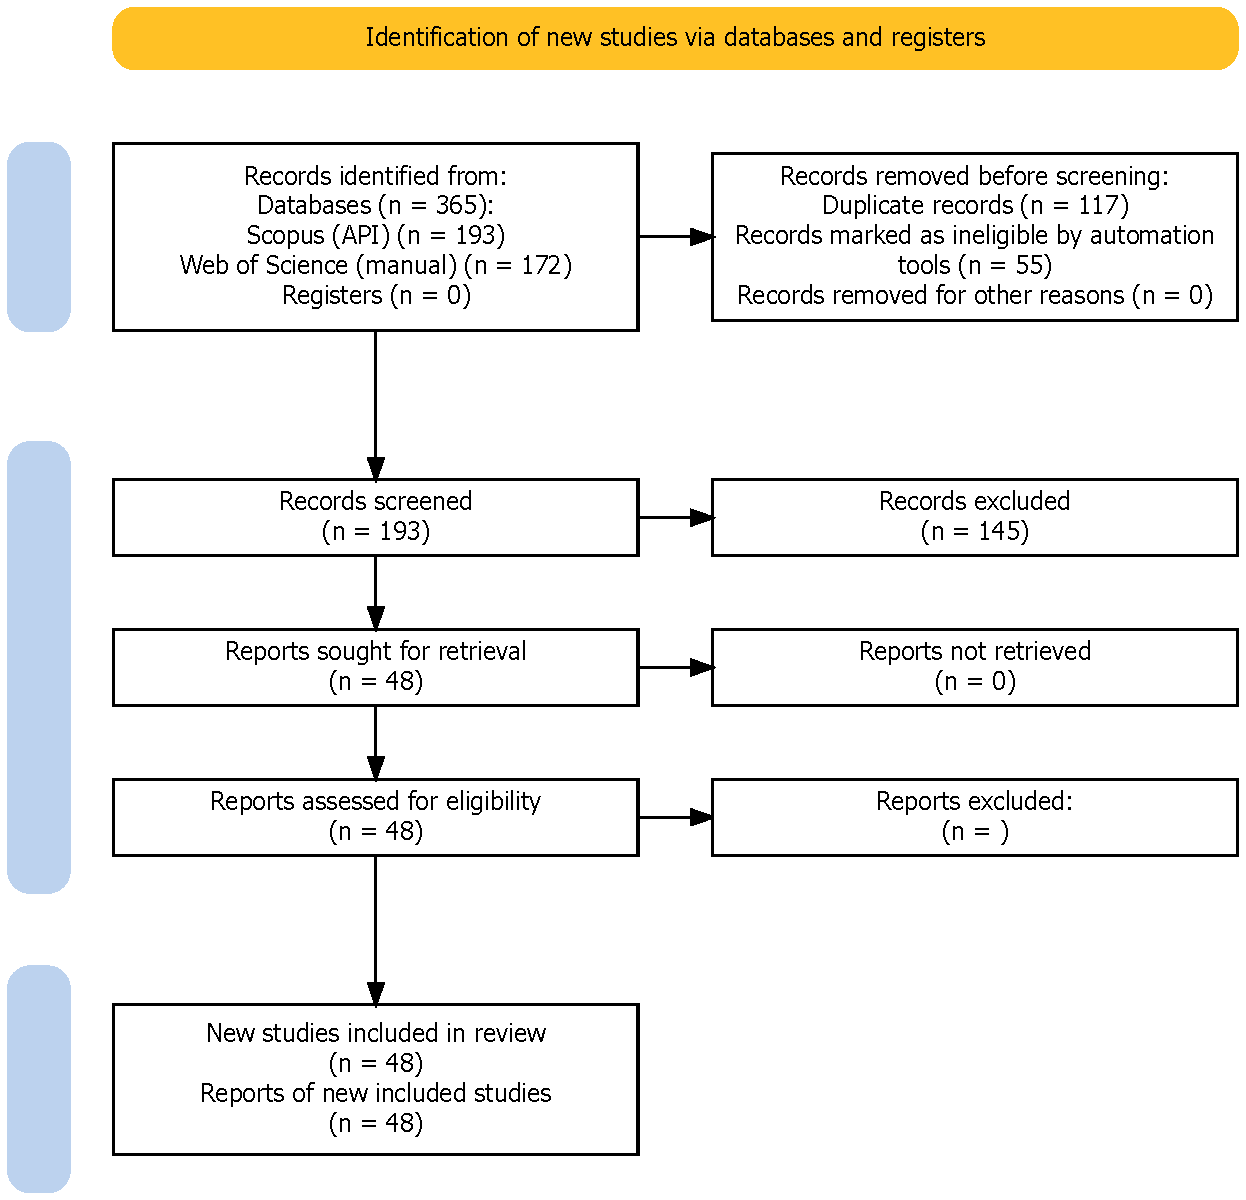
\includegraphics[width=0.68\textwidth]{3-FIGURAS/prisma_flowdiagram_artigo2_en.pdf}
\caption{PRISMA 2020 flow diagram mapping the systematic search, screening restrictions, and deduplication across databases}
\label{fig:prisma-flow}
\end{figure}

The protocol was pre-registered on the OSF Registries platform (DOI: \url{https://doi.org/10.17605/OSF.IO/HE8KT}), and the conduct followed the recommendations of the Cochrane Handbook \citep{Higgins2019} for data extraction, risk-of-bias assessment, and quantitative synthesis.

\subsection{Conceptual framework}
\label{sec:framework}

The biocultural vulnerability of traditional socioecological knowledge was modeled as a multidimensional latent construct, grounded in the convergence between the taxonomy of risks of traditional knowledge erosion \citep{Agrawal2002}, the resilience indicators of socioecological systems \citep{Folke2016}, and vulnerability dimensions identified in the literature. Although the construct was conceived for Traditional Agricultural Knowledge and Systems (TAKS), the empirical parameterization incorporated evidence from communities holding traditional knowledge in a broad sense, including farmers, indigenous peoples, pastoralists, and rural conservation communities distributed across four biogeographic regions (Europe, Africa, the Caribbean, and South America), so as to ensure sufficient contextual variability for the identification of moderators.

The framework posits that aggregate vulnerability results from the interaction of eight functional dimensions ($V_1$--$V_8$), quantifiable through proxy indicators from the empirical literature (Table~\ref{tab:proxies}).

\subsection{Eligibility criteria (PICOS)}
\label{sec:picos}

The eligibility criteria followed the PICOS framework (Table~\ref{tab:picos}).

\begin{table}[htbp]
\caption{PICOS framework (eligibility criteria for the meta-analysis of biocultural vulnerability dimensions).}
\label{tab:picos}
\centering
\small
\begin{tabular}{p{3.5cm} p{9.5cm}}
\toprule
\textbf{Element} & \textbf{Description} \\
\midrule
P (Population) & Communities holding traditional socioecological knowledge, including traditional farmers, indigenous communities, pastoralists, and rural conservation communities, located in tropical, subtropical, and temperate regions. \\
I (Intervention) & Safeguarding practices, structured documentation, heritage registration, legal protection, community knowledge governance, intergenerational transmission revitalization programs, ethnobotanical surveys, seed system assessments, sacred site conservation, post-perturbation food security assessments, sociolinguistic surveys, or climate exposure records, provided they involve measurement of indicators related to the vulnerability dimensions ($V_1$--$V_8$). \\
C (Comparison) & The reference group varied according to the completeness of reported data. In studies with complete quantitative data (Tier~1), the control group corresponded to communities without formal safeguarding interventions or to pre-intervention conditions in before-after designs, with explicit means and standard deviations for both groups. In studies with test statistics without raw data (Tier~2), the contrast between groups was already encoded in the p-value reported by the original study. In studies with narrative or semi-quantitative evidence (Tiers~3 and 4), the reference group was a neutral condition inferred by the coder from the study context, against which the direction of change was judged. In the absence of an explicit control group in any tier, comparison between contrasting subgroups within the same study (age brackets, gender, education level, distance to market) was admitted. \\
O (Outcomes) & Quantitative indicators of biocultural vulnerability operationalized as proxies for the coded dimensions ($V_1$--$V_8$), including proportion of practicing youth, species diversity indices, practice endemism indicators, formal registration rates, legal protection metrics, organizational vitality indicators, linguistic vitality scores, proportion of marketed production, and exposure indices to extreme climatic events (Table~\ref{tab:proxies}). \\
S (Study design) & Comparative empirical studies (cross-sectional with identifiable comparison group or longitudinal before-after), published between 2016 and 2026 in English, Portuguese, or Spanish, reporting quantitative data or semi-quantitative evidence convertible according to the multi-tier protocol described below. \\
\bottomrule
\end{tabular}
\end{table}

The operationalization of the Outcomes component admitted five tiers of evidence in decreasing order of precision, ranging from continuous indicators with complete variances (Tier~1) to directional qualitative judgments converted into synthetic $lnRR$ (Tier~4), recognizing that biocultural safeguarding interventions rarely permit controlled randomization \citep{Shadish2002}.

\subsection{Search strategy and databases}
\label{sec:search}

Bibliographic records were retrieved from Scopus and Web of Science Core Collection using a search strategy comprising three semantic blocks connected by AND (internal variations by OR), in English, Portuguese, and Spanish. The population block included \textit{traditional agricultural system}, \textit{traditional ecological knowledge}, \textit{indigenous farming}, \textit{quilombola}, \textit{smallholder}, \textit{agrobiodiversity}, \textit{agroecology}, and equivalents. The intervention block comprised \textit{safeguard*}, \textit{documentation}, \textit{heritage registration}, \textit{legal protection}, \textit{intangible heritage}, \textit{biocultural conservation}, \textit{community governance}, and equivalents. The outcome block included \textit{vulnerability}, \textit{erosion}, \textit{knowledge loss}, \textit{intergenerational transmission}, \textit{biodiversity index}, \textit{cultural complexity}, \textit{documentation status}, and equivalents.

Searches were supplemented by backward and forward snowballing (Google Scholar). Records exported in BibTeX format were unified and deduplicated using the \textit{revtools} package \citep{Westgate2019}.

\subsection{Screening and selection}
\label{sec:screening}

Prior to formal screening, the two reviewers conducted a pilot calibration exercise with a random sample of 50 records to standardize the interpretation of eligibility criteria and reduce systematic disagreements. Discrepancies identified in the pilot were discussed until operational consensus was reached, and the resulting agreement exceeded the substantial agreement threshold ($\kappa \geq 0.61$), enabling the initiation of full-scale screening.

Screening was conducted in two phases by two independent reviewers. In the title and abstract phase, records were assessed against the PICOS criteria, with discrepancies resolved by consensus or consultation with a third reviewer. In the full-text phase, adequacy to eligibility criteria, data availability for extraction, and absence of sample overlap were verified.

Narrative reviews, book chapters, editorials, and reports without comparative data were excluded. Publications with exclusively qualitative evidence but containing directional judgments on changes in vulnerability indicators (increase, stability, or decrease) were retained as Tier~3 or Tier~4 according to the multi-tier protocol. When data were reported in insufficient format (means without variance or graphical data), authors were contacted before reclassification. The complete flow is documented in the PRISMA~2020 diagram.

\subsection{Functional classification of vulnerability dimensions and proxy variables}
\label{sec:dimensions}

Extracted indicators were organized into eight functional dimensions of biocultural vulnerability (Table~\ref{tab:proxies}).

\begin{table}[htbp]
\caption{Biocultural vulnerability dimensions ($V_1$--$V_8$), proxy variables, units of measurement, and evidence availability in the corpus.}
\label{tab:proxies}
\centering
\scriptsize
\begin{tabular}{p{0.7cm}p{2.2cm}p{4.0cm}p{2.0cm}p{1.3cm}}
\toprule
\textbf{Dim.} & \textbf{Designation} & \textbf{Proxy variables (extractable indicators)} & \textbf{Unit} & \textbf{Avail.} \\
\midrule
$V_1$ & Intergenerational Erosion and Migration & Proportion of youth ($<$ 35 years) with knowledge mastery; active transmission rate; net youth migration balance; proportion of resident youth engaged in agriculture & \%, events$\cdot$yr$^{-1}$, score & High \\
\addlinespace
$V_2$ & Biocultural Complexity and Uniqueness & Managed species richness (Shannon $H'$, Simpson $1-D$); number of local varieties; coded soil-plant interactions; $\beta$-diversity of practices (Jaccard, Bray-Curtis); endemism of varieties; proportion of exclusive practices; seed network connectivity & index, count, \% & High \\
\addlinespace
$V_3$ & Documentation Status & Number of knowledge items with formal registration (inventories, audiovisual); completeness of technical records; digitization rate of collections & count, \% & Moderate \\
\addlinespace
$V_4$ & Legal and Land Tenure Vulnerability & Number of formal protection mechanisms (GI, collective mark, IPHAN registration); existence of community protocol; regulatory gap; existence of collective land title; pending land conflicts & count, binary, ordinal & Low \\
\addlinespace
$V_5$ & Social Organization and Governance & Number of active knowledge holders; frequency of community meetings; vitality of governance protocols; proportion of women in decision-making positions regarding genetic resources & count, events$\cdot$mo$^{-1}$, score, \% & Moderate \\
\addlinespace
$V_6$ & Linguistic Vitality & EGIDS level (0--10); proportion of speakers $<$ 30 years; number of active ethnotaxonomic terms & ordinal, \%, count & Low \\
\addlinespace
$V_7$ & Market Integration & Proportion of production destined for sale; non-agricultural income/total income ratio; replacement rate of landrace varieties by commercial cultivars; distance to market & \%, ratio, km & Low \\
\addlinespace
$V_8$ & Climatic Exposure & SPI (Standardized Precipitation Index); temperature anomaly; frequency of extreme events (drought, flood); WOCAT \S6.3 score & index, $^\circ$C, events$\cdot$yr$^{-1}$, ordinal & Low \\
\bottomrule
\end{tabular}
\end{table}

$V_1$ (Intergenerational Erosion and Migration) captures the discontinuity in vertical knowledge transmission through two mechanistically distinct pathways \citep{ReyesGarcia2013}: acculturation, understood as the in situ replacement of endogenous practices by patterns of the dominant culture \citep{GomezBaggethun2013}, and emigration of knowledge holders, whose co-occurrence with knowledge erosion has been documented in at least five independent studies in the corpus \citep{Tran2025,Moller2023,Bastos2022,VazquezDelfin2022,Aniah2019}. $V_2$ (Biocultural Complexity and Uniqueness) integrates the richness of ecological interactions encoded in traditional systems \citep{Jarvis2008,Brush2004} and the geographic exclusivity of practices, quantified by $\beta$-diversity indices, endemism rates of local varieties, and seed network connectivity between communities \citep{Sibanda2025}. The institutional dimensions $V_3$ (Documentation Status) and $V_4$ (Legal and Land Tenure Vulnerability) measure, respectively, the degree of formal registration and the exposure to misappropriation coupled with land tenure insecurity, with data drawn from heritage program assessments when these contained a comparison group. $V_5$ (Social Organization and Governance) quantifies the vitality of community governance structures \citep{Ostrom1990,Pretty2003} and incorporates women's participation in genetic resource management as an indicator of inclusive governance \citep{Sibanda2025,RomeroSilva2026,MugiNgenga2016}. $V_6$ (Linguistic Vitality) measures the degree of active transmission of vernacular languages bearing ethnotaxonomic terminology, quantifiable by the EGIDS scale \citep{LewisSimons2010} and the VITEK index \citep{ZentMaffi2009}, whose decline entails dissolution of the classification system that underpins practical knowledge \citep{CamaraLeret2021}. $V_7$ (Market Integration) quantifies the pressure to replace landrace varieties with commercial cultivars and the productive reorientation toward sales circuits that decouple cultivation from the logic of socioecological management \citep{Godoy2005,ReyesGarcia2013}. $V_8$ (Climatic Exposure) captures the frequency and intensity of climatic perturbations that force the abandonment of traditional adaptive practices, altering cropping calendars and compromising the viability of local varieties \citep{Savo2016}.

\subsection{Diagnosis of evidence availability and analytical strategy by dimension}
\label{sec:diagnosis}

The analytical strategy adjusted model complexity to evidence density by dimension (Online Resource~4). According to \citet{Borenstein2009}, dimensions with $k \geq 10$ would receive full meta-analysis (subgroups and meta-regression), while dimensions with $k < 10$ would be treated with an exploratory strategy. After multi-tier integration, five dimensions ($V_1$--$V_5$) reached $k = 37$ and three dimensions ($V_6$--$V_8$) reached $k = 47$, enabling confirmatory analysis for all eight dimensions. Dimensions $V_6$ (linguistic vitality), $V_7$ (market integration), and $V_8$ (climatic exposure) were coded exclusively from Tier~3 and Tier~4 evidence (direction and intensity without explicit inferential statistics).

\subsection{Data extraction protocol}
\label{sec:extraction}

Extraction followed a three-block protocol using a standardized form completed by two independent reviewers.

The study metadata block recorded author, publication year, DOI, country, biogeographic region (Africa, South America, the Caribbean, Europe), community type (farmers, indigenous, pastoralists, rural), intervention type, intervention duration in years, and study design (comparative cross-sectional, longitudinal before-after).

The effect size calculation block recorded, for each paired comparison, the assigned functional dimension ($V_1$--$V_8$), the specific proxy indicator (per Table~\ref{tab:proxies}), and the unit of measurement. The completeness of subsequent fields determined the record's classification under the multi-tier protocol. For Tier~1 studies, we extracted the intervention group mean ($\bar{X}_T$), intervention group standard deviation ($SD_T$), intervention group sample size ($n_T$), control group mean ($\bar{X}_C$), control group standard deviation ($SD_C$), and control group sample size ($n_C$). For Tier~2 studies, we extracted the p-value or test statistic, sample sizes, and effect direction. For Tiers~3 and 4 studies, the coded direction ($+1$, $0$, or $-1$) and perceived intensity (1, 2, or 3) were recorded according to the ordinal coding protocol. When studies reported standard error ($SE$), conversion to standard deviation was performed as
%
\begin{equation}
SD = SE \times \sqrt{n}
\label{eq:sd-ep}
\end{equation}

\noindent When only confidence intervals were available, means and standard deviations were estimated following \citet{Betancur2022}. Data presented exclusively in figures were digitized using WebPlotDigitizer v4.3 \citep{Rohatgi2020}. When studies reported results for multiple communities or time periods, data were extracted separately for each condition.

The moderator block recorded intervention type (ethnobotanical survey, farmer perception, post-perturbation food security, sacred grove conservation, seed system assessment), biogeographic region (Africa, South America, the Caribbean, Europe), and community type (farmers, indigenous, pastoralists, rural).

\subsection{Multi-tier evidence integration protocol}
\label{sec:multitier}

The 48 eligible studies were classified into five evidence tiers according to the completeness of reported data, with calibrated conversions and explicit uncertainty propagation. Studies with complete means, standard deviations, and sample sizes (Tier~1) permitted direct calculation of $lnRR$ and $v_i$ (Equations~\ref{eq:lnrr} and~\ref{eq:vi}).

When only numerical p-values and sample sizes were identifiable (Tier~2a), the effect size was obtained through the chain $p \rightarrow z \rightarrow d \rightarrow lnOR \rightarrow lnRR$, operationalized by the sequence of conversions expressed in Equations~\ref{eq:z-conv}--\ref{eq:lnrr-conv}.
%
\begin{align}
z &= \Phi^{-1}(1 - p/2) \label{eq:z-conv} \\
d &= z \cdot \sqrt{\frac{1}{n_T} + \frac{1}{n_C}} \label{eq:d-conv} \\
lnOR &= \frac{d \cdot \pi}{\sqrt{3}} \label{eq:lnor-conv} \\
lnRR &= lnOR - \ln\!\bigl(1 - p_0 + p_0 \cdot e^{lnOR}\bigr) \label{eq:lnrr-conv}
\end{align}

\noindent Equation~\ref{eq:z-conv} converts the two-tailed p-value to the standard normal quantile $z$; Equation~\ref{eq:d-conv} converts $z$ to $d$ \citep{Borenstein2009}; Equation~\ref{eq:lnor-conv} transforms $d$ to $lnOR$ \citep{Hasselblad1995}; Equation~\ref{eq:lnrr-conv} converts $lnOR$ to $lnRR$ \citep{Zhang1998} with $p_0 = 0.5$. When the median $CV$ from Tier~1 studies in the same dimension was available, the alternative conversion
%
\begin{equation}
lnRR \approx d \cdot CV_{ref}
\label{eq:lnrr-cv}
\end{equation}

\noindent from \citet{Lajeunesse2011} was employed.

The same chain was applied to studies that reported test statistics without explicit p-values (Tier~2b), adopting conservative thresholds ($p = 0.05$ for moderate/strong effects, $p = 0.10$ for weak effects). Studies that presented tabulated numerical comparisons without test statistics (Tier~3) and studies with exclusively narrative conclusions (Tier~4) were submitted to independent ordinal coding by two reviewers, with additional variance inflation ($\times 1.5$) for the qualitative case.

The uncertainty associated with each conversion was propagated by inflating the standard error as
%
\begin{equation}
SE_{adj} = SE \cdot \sqrt{1 + \sigma^2_{conv}}
\label{eq:se-adj}
\end{equation}

\noindent where $\sigma_{conv}$ assumes increasing values by tier ($0.15$ for Tier~2a, $0.25$ for Tier~2b, $0.35$ for Tier~3, and $0.50$ for Tier~4). Robustness was assessed through meta-regression with a \textit{direct evidence} indicator (Tier~1 vs.\ others) and through sensitivity analysis restricted to the Tier~1 subset.

\subsection{Ordinal coding and conversion to synthetic \texorpdfstring{$lnRR$}{lnRR}}
\label{sec:coding}

For records classified as Tier~3 and Tier~4, two independent reviewers coded each comparison along two dimensions, following a coding protocol with prior calibration ($\kappa \geq 0.61$). The effect direction dimension assigned values of $+1$ (vulnerability aggravated), $0$ (neutral), or $-1$ (vulnerability reduced) based on interpretation of the original text. The intensity dimension classified perceived magnitude as weak (1), moderate (2), or strong (3) based on narrative emphasis, reported statistical significance (when available), and amplitude of described change.

Ordinal scores were converted to synthetic $lnOR$ through mapping to fixed quantiles of the logit-normal distribution with variance $\pi^2/3 \approx 3.29$ \citep{Hasselblad1995}, yielding $lnOR$ values of $-0.405$ (weak), $+0.405$ (moderate), and $+1.386$ (strong), multiplied by the coded direction. The subsequent conversion from $lnOR$ to $lnRR$ employed the \citet{Zhang1998} transformation with $p_0 = 0.5$, and the variance of the synthetic $lnRR$ incorporated both the fixed logistic variance ($\pi^2/3$) and the conversion uncertainty inflation.

The sign convention adopted operates as a scalar multiplier on the absolute magnitude of the effect, such that the resulting $lnRR$ preserves directional interpretation throughout the conversion chain. Values of $lnRR > 0$ indicate that the exposed group exhibits vulnerability indicators superior to the reference group, corresponding to worsening of the biocultural condition, whereas $lnRR < 0$ indicates a protective effect, with more favorable indicators in the exposed group. The operational definition of the reference group varied by evidence tier.

In Tier~1 studies, the control group corresponded to communities without formal safeguarding interventions or to pre-intervention conditions in before-after designs, with explicit means and standard deviations. In Tier~2 studies, the contrast was already encoded in the test statistic reported by the original study. In Tier~3 and Tier~4 studies, the reference group was a neutral condition inferred by the coder from the narrative context, against which the direction of change ($+1$, $0$, or $-1$) was judged.

\subsection{Missing data treatment and hierarchical structure}
\label{sec:missing}

The composition of the corpus (94\% of records lacking complete means and standard deviations) rendered multiple imputation (MICE) \citep{vanBuuren2011} impracticable; it was replaced by the multi-tier protocol. This approach preserved all 47~eligible studies (363~records, $k = 37$ per dimension for $V_1$--$V_5$ and $k = 47$ for $V_6$--$V_8$). Sensitivity analyses compared estimates from the full model with the Tier~1 subset ($k_{T1} = 3\text{--}5$).

The database was hierarchically structured at three levels \citep{Pustejovsky2022} to control for dependencies arising from multiple comparisons extracted from a single study. Level~1 represented each paired comparison with $lnRR$ and sampling variance; Level~2 grouped observations from the same publication via random effects; Level~3 incorporated fixed moderators and residual between-study variance ($\tau^2$), estimated by REML.

The within-study variance-covariance matrix ($\mathbf{V}_j$) assumed constant correlation $\rho = 0.8$ between pairs of effect sizes from the same study \citep{Pustejovsky2022}, with sensitivity assessed over the interval $[0.5;\; 1.0]$. Robust variance estimation (RVE) with CR2 correction was applied via \textit{clubSandwich} ($\geq$ 0.5.5).

Overall heterogeneity was quantified by Cochran's $Q$ test and the $I^2$ index (Equation~\ref{eq:i2}), interpreted according to the thresholds of \citet{Higgins2003}, wherein $I^2 < 25\%$ indicates low heterogeneity, 25--75\% moderate, and $> 75\%$ high.

\begin{equation}
I^2 = \frac{Q - (k-1)}{Q} \times 100
\label{eq:i2}
\end{equation}

\subsection{Statistical analysis}
\label{sec:stats}

The $lnRR$ was adopted as the effect size metric \citep{Hedges1999}, calculated according to Equation~\ref{eq:lnrr}.

\begin{equation}
lnRR = \ln\left(\frac{\bar{X}_{T}}{\bar{X}_{C}}\right)
\label{eq:lnrr}
\end{equation}

\noindent Values of $lnRR > 0$ indicate improvement of the indicator under intervention, $lnRR < 0$ indicate deterioration, and the back-transformation $(e^{lnRR} - 1) \times 100$ provides the percentage change. The sampling variance was estimated according to Equation~\ref{eq:vi} \citep{Hedges1999}.

\begin{equation}
v_i = \frac{SD_T^2}{n_T \cdot \bar{X}_T^2} + \frac{SD_C^2}{n_C \cdot \bar{X}_C^2}
\label{eq:vi}
\end{equation}

The hierarchical mixed-effects model was fitted with a restricted maximum likelihood (REML) estimator to estimate between-study variance ($\tau^2$), according to Equation~\ref{eq:model}.

\begin{equation}
lnRR_{ij} = \mu + \bm{\beta} \cdot \mathbf{X}_{ij} + u_j + \epsilon_{ij}
\label{eq:model}
\end{equation}

\noindent where $lnRR_{ij}$ is the effect size of observation $i$ in study $j$, $\mu$ is the intercept (overall or per-dimension mean effect), $\bm{\beta} \cdot \mathbf{X}_{ij}$ is the fixed moderator vector, $u_j \sim N(0, \tau^2)$ is the study-level random effect, and $\epsilon_{ij}$ is the residual error.

The prediction interval complemented the 95\% CI \citep{IntHout2016}. Estimates of $\tau^2$ were compared between DerSimonian-Laird and REML \citep{Borenstein2009}.

The sensitivity of estimates to individual studies was assessed through leave-one-out analyses \citep{Viechtbauer2010}.

Publication bias was assessed by the Begg test \citep{Begg1994} and the trim-and-fill method \citep{Duval2000}.

Meta-regressions with fixed moderators (intervention type, biogeographic region, community type) were conducted by dimension; time since intervention was excluded due to the absence of codable data. The omnibus test ($Q_M$) assessed the joint significance of moderators.

All analyses were conducted in R (version 4.5.1) using the \textit{metafor} package (version 4.8-0) \citep{Viechtbauer2010} (hierarchical models, meta-regression), \textit{clubSandwich} \citep{Pustejovsky2022} (RVE with CR2), \textit{meta} (version 8.2-1; forest plots, subgroups), and \textit{dmetar} (influence, sensitivity). The significance level was set at $\alpha = 0.05$.

\subsection{Functional outputs of the meta-analysis}
\label{sec:outputs}

The meta-analysis produced four integrated quantitative outputs: ranking of $\overline{lnRR}$ by dimension, heterogeneity indices ($I^2$, $\tau^2$), meta-regression coefficients for contextual moderators, and 95\% CIs of $lnRR$, enabling ranking of dimension responsiveness and delineation of estimate precision.

For $V_2$ and $V_4$, multi-tier integration raised $k$ to the confirmatory threshold, although the Tier~1 base remains restricted, and estimates should be interpreted with caution.

\subsection{Evidence gap analysis}
\label{sec:gaps}

For each dimension, the number of proxy variables (Table~\ref{tab:proxies}) without sufficient data for $lnRR$ calculation was tallied, producing a missing evidence vector that identifies priority gaps for primary data collection. The indicator-to-dimension mapping is consolidated in Online Resource~3.

Fig.~\ref{fig:methods-flow} synthesizes the complete operational sequence, from the definition of the conceptual framework to the production of functional outputs from the meta-analytic synthesis.

\begin{figure}[H]
\centering
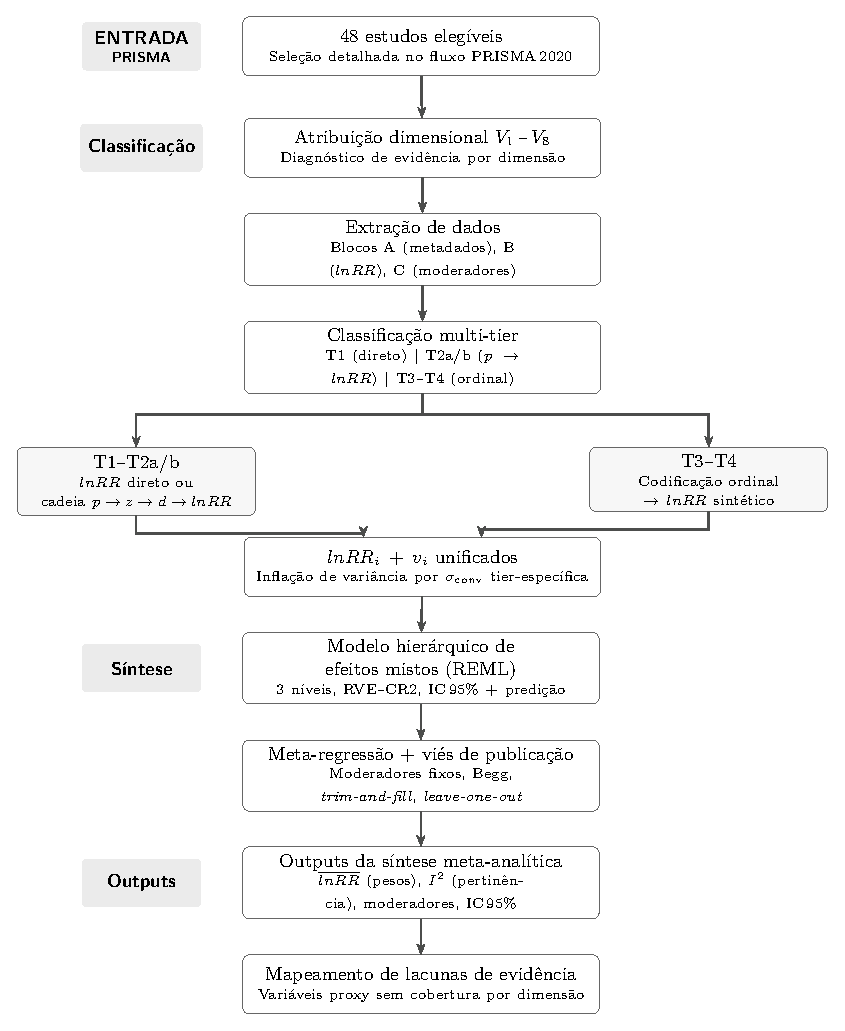
\includegraphics[width=0.82\textwidth]{3-FIGURAS/methods_flowchart.pdf}
\caption{Methodological flowchart integrating the stages of scoping, screening, multi-tier classification, statistical synthesis, and production of functional outputs}
\label{fig:methods-flow}
\end{figure}


%% ============================================================
%% 3. RESULTS AND DISCUSSION
%% ============================================================
\section{Results and Discussion}
\label{sec:results}

\subsection{PRISMA selection flow}
\label{sec:prisma-flow}

The systematic search (2016--2026) retrieved 365 records (193 from Scopus via API, 172 from Web of Science via direct export). Document type and temporal window filters excluded 33 ineligible records (chapters, conferences, and editorials) and 20 records outside the study period, reducing the corpus to 310 candidates. Cross-database deduplication by DOI and title normalization eliminated 117 inter-database duplicates (81\% overlap), resulting in 193 unique records with a net contribution of 27 exclusive Web of Science records.

Semantic screening required the simultaneous presence of descriptors from Blocks~1 (population) and 2 or 3 (intervention/outcomes), reducing the corpus from 193 to 42 records. Fuzzy matching (\textit{stringdist}, OSA method, threshold $= 5$) via \textit{revtools} identified no additional duplicates; however, manual re-screening of 139 records lacking abstracts in the Scopus export recovered six eligible studies \citep{Aswani2020,Bussmann2018,Ghanimi2022,Malapane2024,RodriguezCruz2022,Rodriguez2018}, raising the corpus from 42 to 48 records, bringing total exclusions to 145.

The retention rate of 24.9\% ($48/193$) reflects the specificity of the scope, which requires simultaneous convergence between population evidence, vulnerability measurement, and safeguarding intervention---an intrinsically rare combination in the indexed literature \citep{Agrawal2002}. The exclusion of the 145 records resulted from the convergence of absence of quantitative outcomes (descriptive perspective without comparison groups), thematic misalignment with the safeguarding domain (population blocks without intersection with intervention or outcomes), and predominance of qualitative approaches without extractable statistical parameters for $lnRR$ calculation.

The 48 retained records comprise 46 original articles and two reviews, published between 2016 and 2026, with a predominance of Scopus records ($n = 33$, 68.8\%) and complementary contribution from the Web of Science ($n = 15$, 31.2\%), as detailed in Fig.~\ref{fig:prisma-flow}. One study (ID=36) was excluded during coding due to insufficient data, resulting in 47~final studies.

\subsection{Multi-tier evidence base composition}
\label{sec:tier-composition}

Of the 47 final studies, five (10.6\%) provided complete means and standard deviations (Tier~1, 18~records), seven (14.9\%) reported convertible inferential statistics (Tier~2a: 21~records from $p$-values; Tier~2b: 21~records from ANOVA thresholds), and 35 (74.5\%) contributed exclusively with ordinally coded qualitative evidence (Tier~3: 74~records with cross-tabulations; Tier~4: 88~purely qualitative records). The multi-tier conversion produced 363~records with $lnRR$ and associated variance, totaling $k = 37$ studies per dimension for $V_1$--$V_5$ and $k = 47$ for $V_6$--$V_8$, whose proxy variables (linguistic vitality, market integration, and climatic exposure) were coded exclusively from Tier~3 and Tier~4 evidence (direction and intensity without explicit inferential statistics). All eight dimensions reached the confirmatory threshold of $k \geq 15$, permitting full meta-analysis for the entire set.

\subsection{Meta-analytic synthesis by dimension}
\label{sec:meta-results}

The three-level hierarchical model (observation/study/meta-analysis) with REML estimator and RVE-CR2 (Fig.~\ref{fig:forest-agregado}) indicated that two dimensions exhibited significant effects among the eight operationalized: $V_4$ (legal and land tenure vulnerability) and $V_8$ (climatic exposure).

Legal and land tenure vulnerability ($V_4$) concentrated the only significantly negative effect ($\overline{lnRR} = -0.279$; 95\% CI: $[-0.49;\; -0.06]$; $p < 0.05$), corresponding to a 24.3\% reduction in formal protection indicators. This result is consistent with the disconnect between customary tenure regimes and national intellectual property regulatory frameworks \citep{Santilli2009,Dutfield2004,Cottier2004}. The moderate heterogeneity of this dimension ($I^2 = 30.7\%$; $\tau^2 = 0.171$) signals that the gradient of legal vulnerability is conditioned by regional and institutional factors, explored in the moderator subsection. In contrast, social organization and governance ($V_5$) exhibited a positive trend of 18.7\% ($\overline{lnRR} = +0.172$; 95\% CI: $[-0.05;\; 0.40]$; $p \approx 0.13$), compatible with the hypothesis that safeguarding interventions activate community cohesion mechanisms that translate into greater frequency of transmission events and vitality of governance protocols \citep{Ostrom1990,Berkes2007,Rathwell2015}, although statistical significance was not reached at the global scale.

Climatic exposure ($V_8$) presented the second significant effect of the synthesis ($\overline{lnRR} = +0.280$; 95\% CI: $[0.03;\; 0.53]$; $k = 47$), corresponding to a 32.3\% increase in vulnerability indicators associated with climatic variability, droughts, and extreme events. The negligible heterogeneity ($I^2 \approx 0$; $\tau^2 \approx 0$) indicates that the effect is homogeneously distributed across studies, with a narrow prediction interval (95\% PI: $[0.04;\; 0.52]$) that does not cross zero, supporting the robustness of the estimate. Market integration ($V_7$, $\overline{lnRR} = +0.051$; 95\% CI: $[-0.01;\; 0.11]$; $k = 47$) exhibited a marginal positive trend of 5.3\%, whereas linguistic vitality ($V_6$, $\overline{lnRR} = 0.000$; $k = 47$) registered a null effect, consistent with Dir = 0 coding across all studies for this dimension.

Biocultural complexity and uniqueness ($V_2$), whose two proxy variables per study generate 74 observations with within-study correlation $\rho = 0.8$, exhibited a near-zero effect ($\overline{lnRR} = +0.017$; 95\% CI: $[-0.09;\; 0.12]$; $I^2 = 3.6\%$), with the lowest heterogeneity among all dimensions. Intergenerational erosion ($V_1$, $\overline{lnRR} = -0.017$; $I^2 = 14.8\%$) and documentation status ($V_3$, $\overline{lnRR} = +0.007$; $I^2 = 7.6\%$) also remained near zero, consistent with the protective potential of in situ conservation practices \citep{Brush2004}. The wide prediction intervals for all dimensions (e.g., $V_4$ with 95\% PI of $[-1.11;\; 0.56]$) delineate the expected variability across future contexts without altering the direction of the main effect observed for $V_4$ (Fig.~\ref{fig:forest-agregado}).


\begin{figure}[H]
\centering
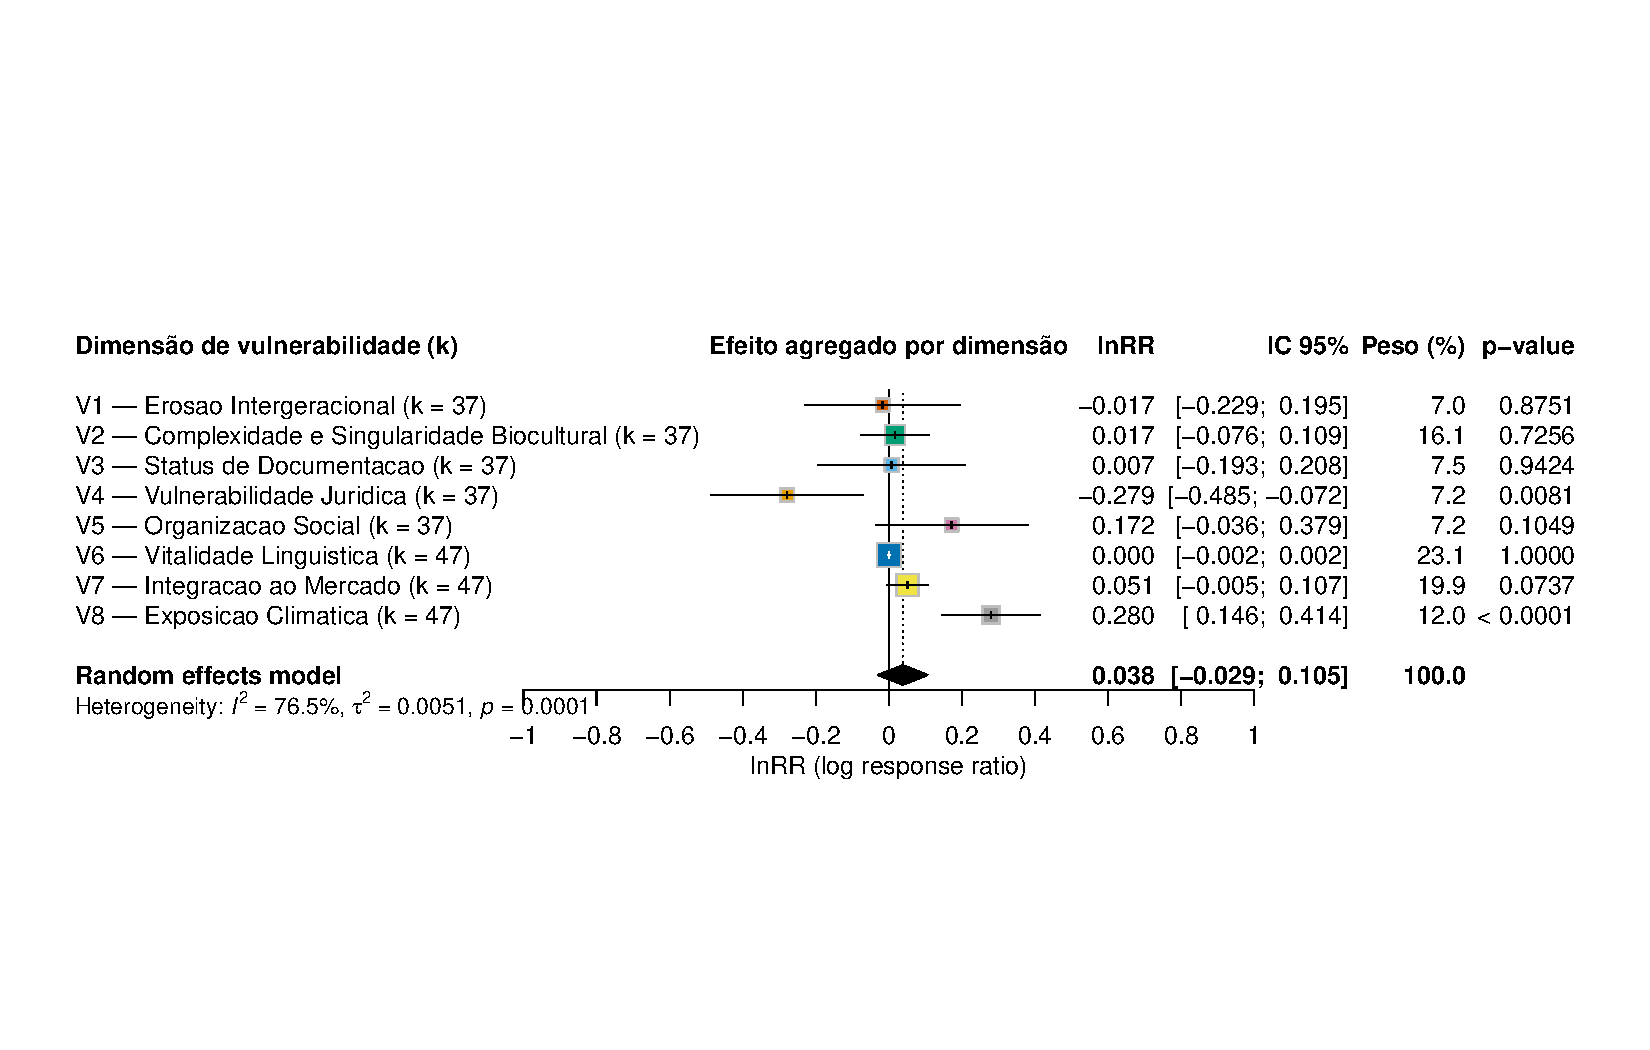
\includegraphics[width=0.95\textwidth]{3-FIGURAS/forest_agregado_V1_V8.pdf}
\caption{Aggregated forest plot of the eight vulnerability dimensions ($V_1$--$V_8$). $V_1$--$V_5$ comprise $k = 37$ studies and $V_6$--$V_8$ comprise $k = 47$ studies per dimension. Points represent the $\overline{lnRR}$ with 95\% CI (solid lines) and prediction interval (dashed lines). The dashed vertical line indicates the null effect}
\label{fig:forest-agregado}
\end{figure}

\subsection{Meta-regression and moderators}
\label{sec:meta-regression}

$V_4$ (legal and land tenure vulnerability) was the only dimension whose heterogeneity was partially attributable to the contextual moderators tested (intervention type, biogeographic region, and community type; $Q_M = 3.82$; $p = 0.070$; $I^2 = 30.7\%$). For the remaining dimensions, $Q_M$ values did not reach significance ($V_1$: $Q_M = 2.18$, $p = 0.20$; $V_2$: $Q_M = 1.57$, $p = 0.09$; $V_5$: $Q_M = 1.48$, $p = 0.35$; $V_3$: $Q_M = 1.20$, $p = 0.46$; $V_6$--$V_8$: $Q_M \approx 0$, $p = 1.00$), which does not preclude that individual coefficients for $V_1$--$V_6$ reveal relevant mechanistic patterns.

The continental gradient modulates the magnitude of the legal effect with an asymmetry consistent with distinct institutional regimes (Fig.~\ref{fig:meta-reg-regiao}). For $V_4$, South America ($k = 12$; $\overline{lnRR} = -0.464$; 95\% CI: $[-0.77;\; -0.16]$) and Asia ($k = 4$; $\overline{lnRR} = -0.557$; 95\% CI: $[-1.04;\; -0.07]$) concentrated significantly negative effects, a pattern interpretable as reflecting contexts where land tenure pressure on traditional territories converges with regulatory frameworks that inadequately recognize customary tenure.

Conversely, Africa ($k = 10$; $\overline{lnRR} = -0.061$) and Europe ($k = 6$; $\overline{lnRR} = -0.125$) maintained intervals compatible with neutrality, suggesting that regional compensatory mechanisms (community seed custodianship, formalized ethnobotanical networks) attenuate the legal erosion observed at other latitudes.

\begin{figure}[htbp]
\centering
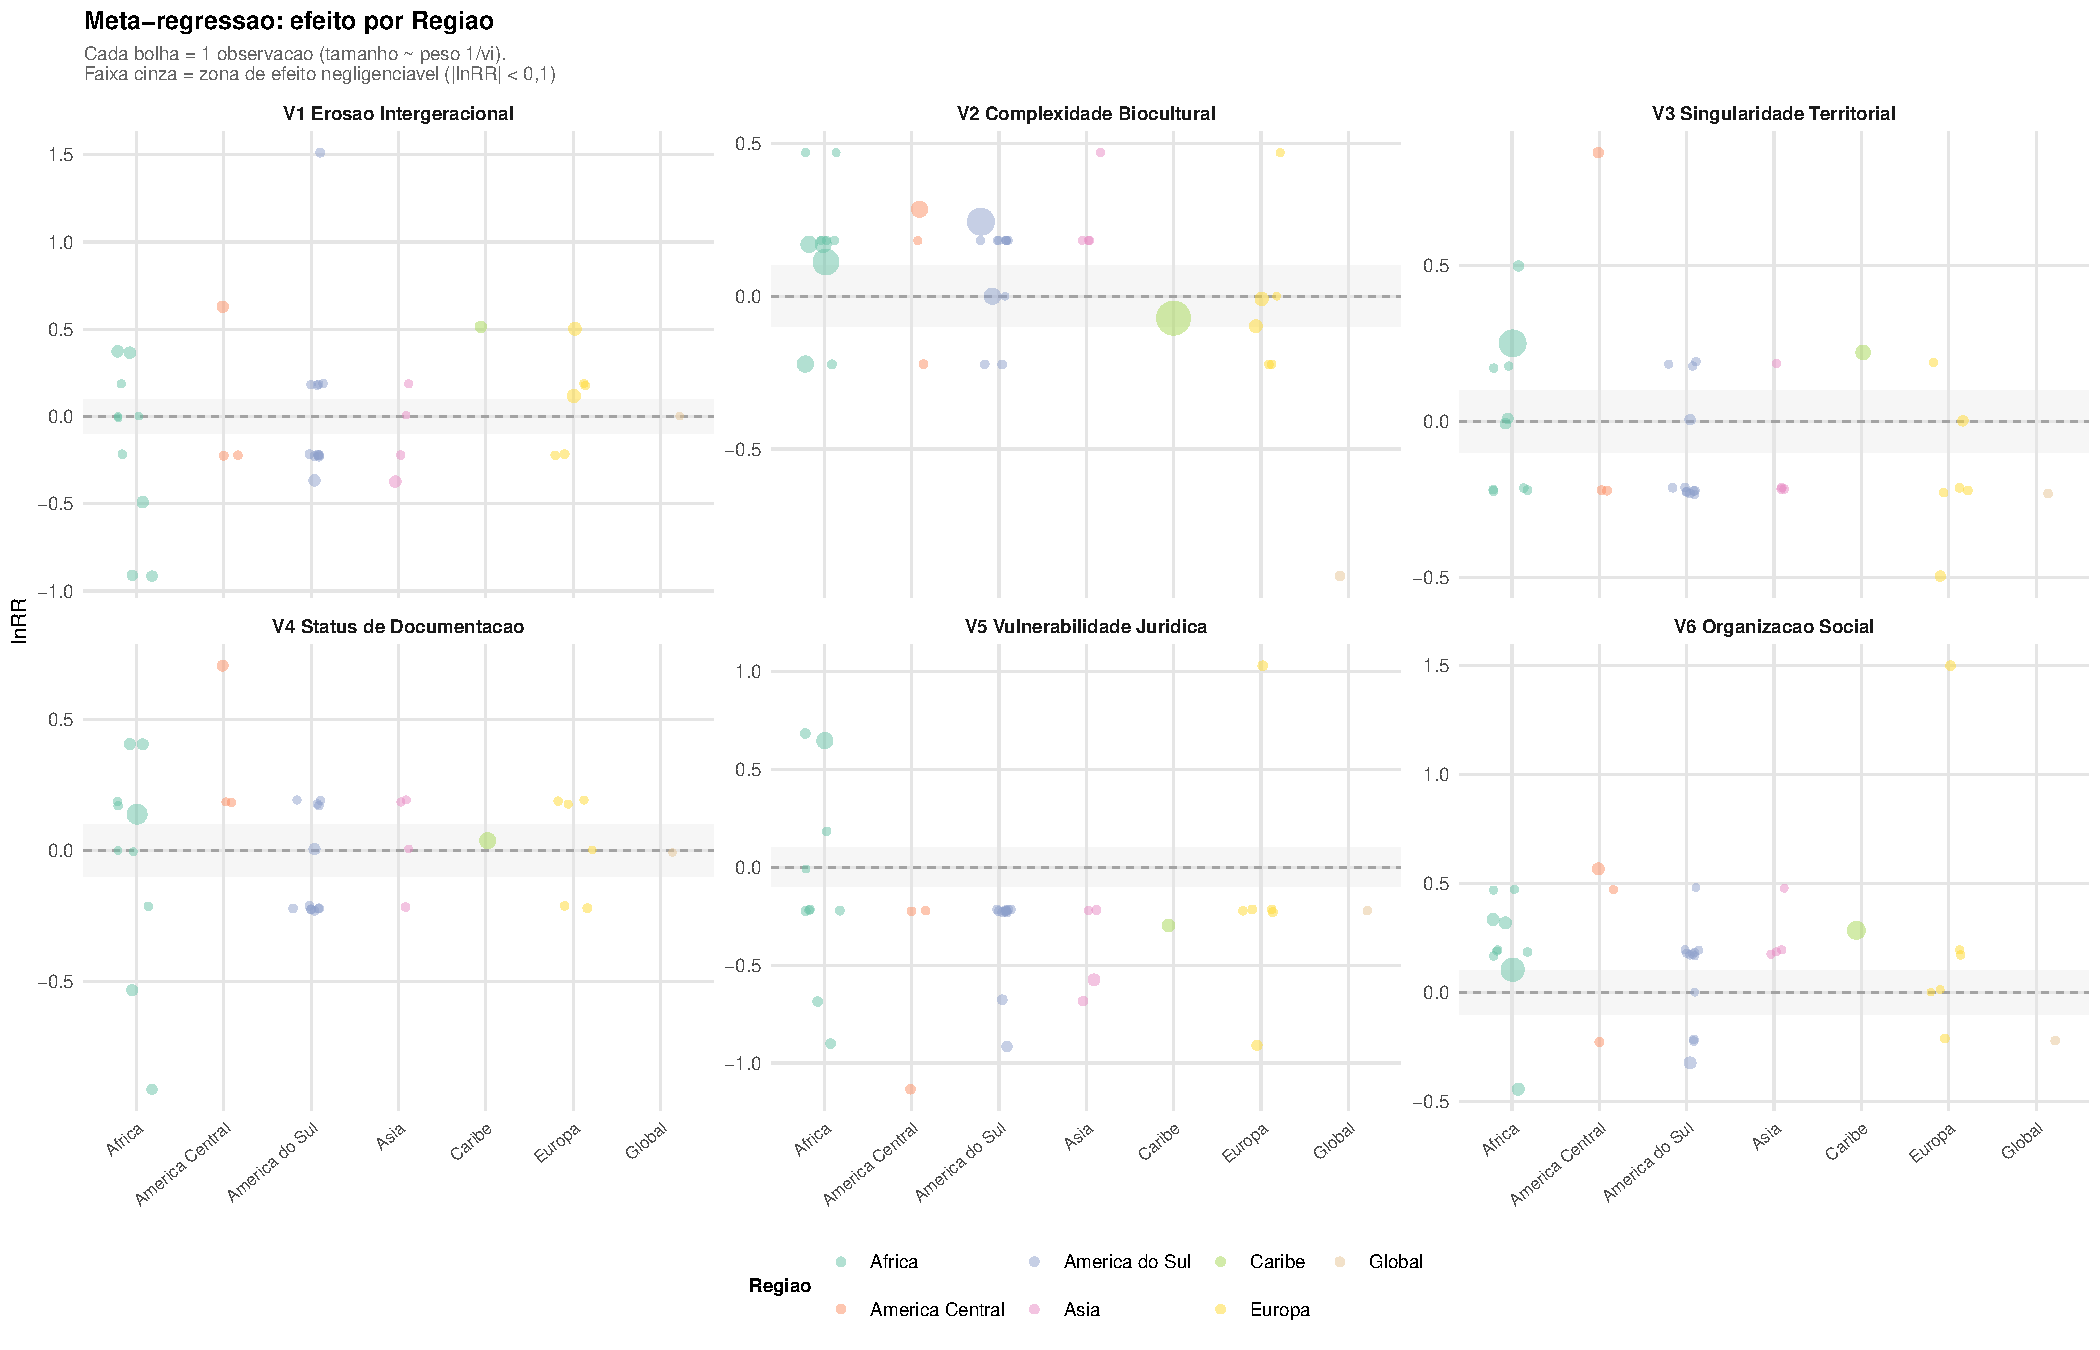
\includegraphics[width=0.95\textwidth]{3-FIGURAS/meta_regressao_regiao.pdf}
\caption{Meta-regression: effect by biogeographic region for each vulnerability dimension. Each bubble represents a study-dimension observation, with size proportional to weight ($1/v_i$). The gray band delineates the negligible effect zone ($|lnRR| < 0.1$)}
\label{fig:meta-reg-regiao}
\end{figure}

Farming communities exhibited, for $V_4$ (Fig.~\ref{fig:meta-reg-comunidade}), the most pronounced negative effect ($k = 12$; $\overline{lnRR} = -0.395$; 95\% CI: $[-0.73;\; -0.06]$), a context in which conventional agricultural policies collide with customary tenure regimes, exacerbating tenure insecurity. Indigenous communities, in contrast, maintained a negative effect without significance ($\overline{lnRR} = -0.241$; 95\% CI: $[-0.60;\; 0.12]$), possibly because specific regulatory frameworks (Nagoya protocols, collective intellectual property legislation) provide partial protection that does not extend to traditional farmers lacking formal ethno-territorial recognition. For $V_5$ (social organization and governance), rural communities exhibited the largest positive trend ($k = 7$; $\overline{lnRR} = +0.688$; 95\% CI: $[-0.26;\; 1.63]$), suggesting that collective organization in rural contexts may function as a compensatory mechanism in the face of vulnerability in other dimensions, although the width of the interval warrants caution.

\begin{figure}[htbp]
\centering
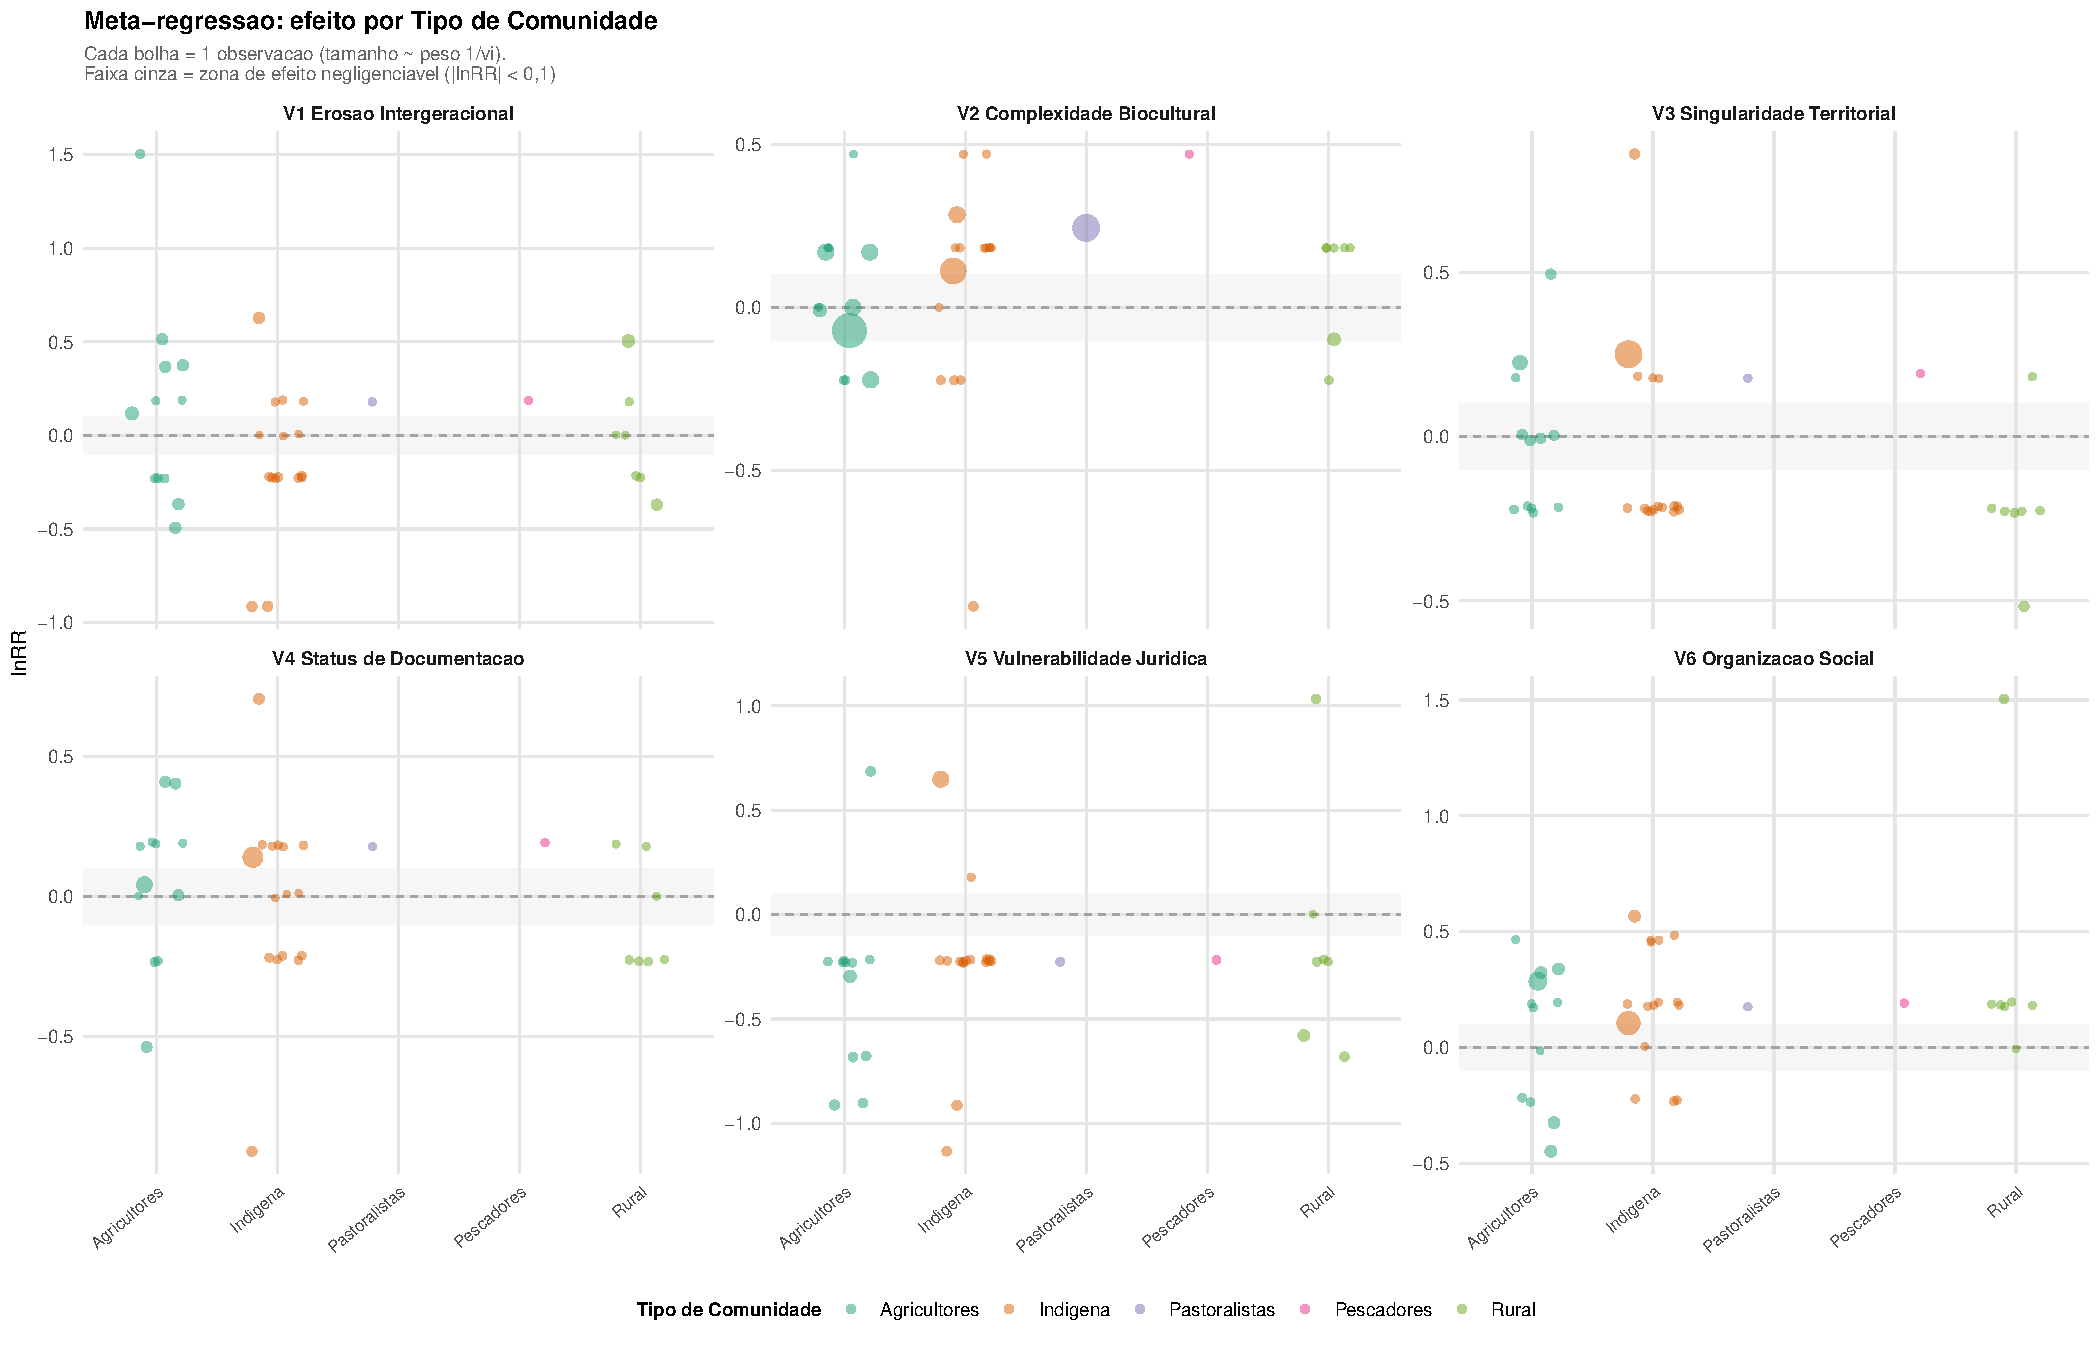
\includegraphics[width=0.95\textwidth]{3-FIGURAS/meta_regressao_comunidade.pdf}
\caption{Meta-regression: effect by community type for each vulnerability dimension. Each bubble represents a study-dimension observation, with size proportional to weight ($1/v_i$). The gray band delineates the negligible effect zone ($|lnRR| < 0.1$)}
\label{fig:meta-reg-comunidade}
\end{figure}

For $V_4$ (legal vulnerability, Fig.~\ref{fig:meta-reg-intervencao}), studies centered on the erosion of traditional knowledge ($\beta = +1.284$; $p = 0.060$) and flood knowledge ($\beta = +0.753$; $p = 0.078$) exhibited a worsening trend, consistent with the hypothesis that these investigations capture erosive processes already underway, whereas agroforestry assessments ($\beta = -0.673$; $p = 0.062$) suggested a marginal protective effect. For $V_5$ (social organization), sacred grove conservation ($\beta = +1.496$; $p = 0.014$) and biocultural conservation ($\beta = +0.416$; $p = 0.022$) exhibited significant positive effects, indicating that interventions anchored in symbolic territories activate community cohesion mechanisms, while ecological knowledge indicators exhibited a negative effect ($\beta = -0.919$; $p < 0.001$), suggesting that mere species cataloging does not translate into tangible social gains. For $V_6$ (linguistic vitality), sacred grove conservation ($\beta = +1.407$; $p = 0.001$), followed by traditional knowledge on erosion ($\beta = +0.643$; $p = 0.009$) and flood knowledge ($\beta = +0.455$; $p = 0.020$), replicated the territorial effect pattern observed for $V_5$, suggesting that strategies linking normative reinforcement to ritual practices may simultaneously activate social cohesion and cultural vitality. For $V_2$ (biocultural complexity and uniqueness), despite the non-significant omnibus test, five individual coefficients reached $p < 0.10$, notably \textit{home garden knowledge transmission} ($\beta = -0.783$; $p = 0.019$) and sacred grove conservation ($\beta = -0.658$; $p = 0.029$), indicating that in situ conservation interventions produce detectable protective effects even when overall heterogeneity is low ($I^2 = 3.6\%$). The reduced sample sizes per subgroup ($k = 1$--$5$), however, limit the generalizability of these findings.

\begin{figure}[htbp]
\centering
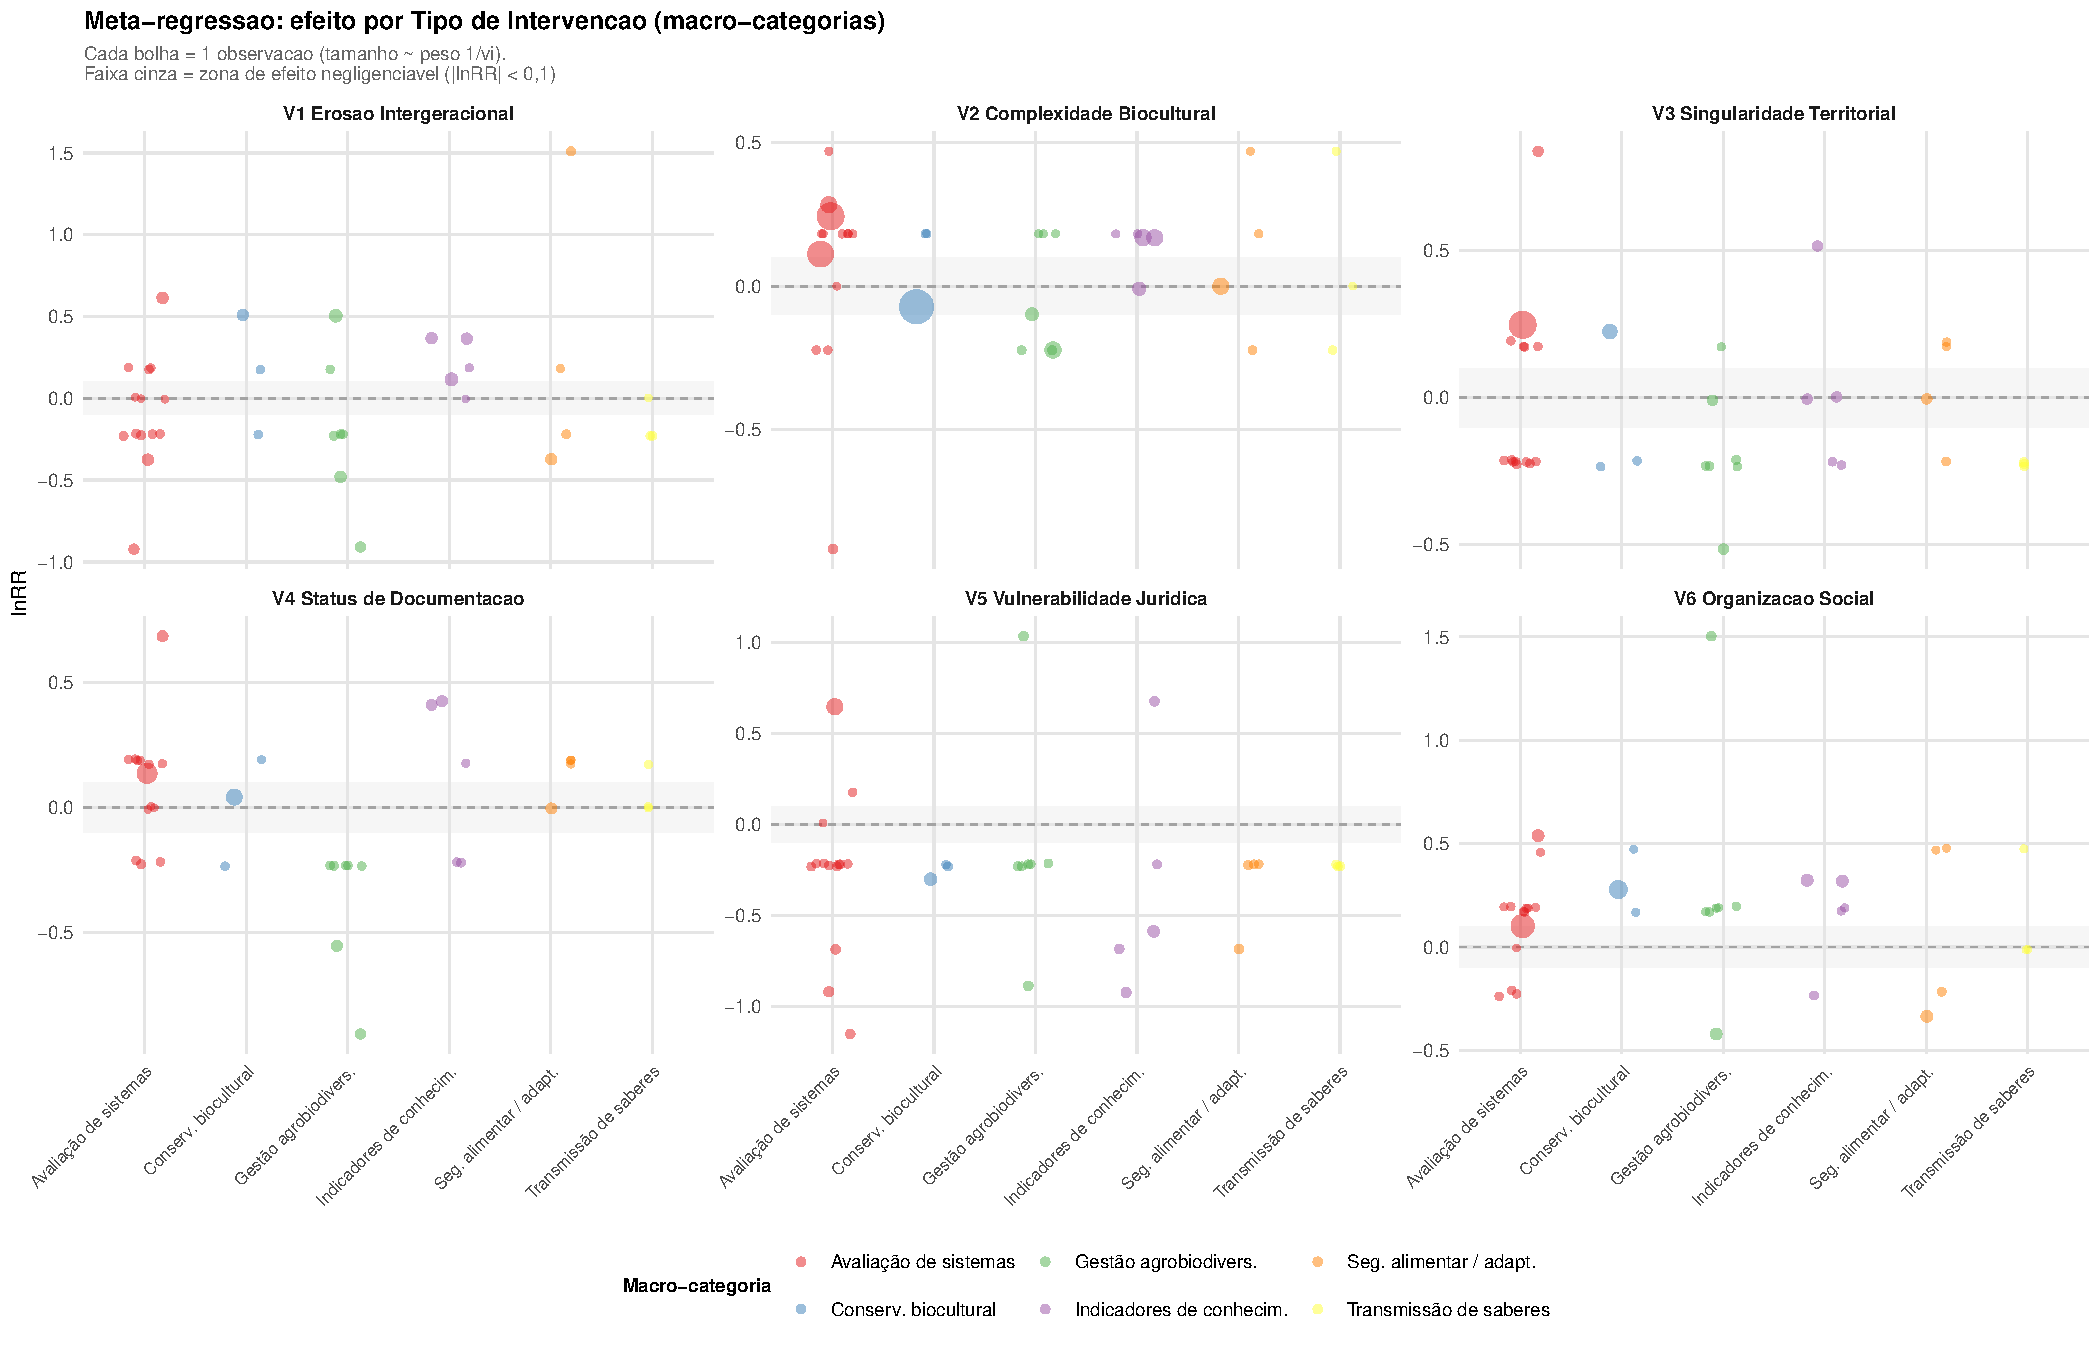
\includegraphics[width=0.95\textwidth]{3-FIGURAS/meta_regressao_intervencao.pdf}
\caption{Meta-regression: effect by intervention macro-category for each vulnerability dimension. Each bubble represents a study-dimension observation, with size proportional to weight ($1/v_i$). The original 27 categories were grouped into six macro-categories for visualization purposes}
\label{fig:meta-reg-intervencao}
\end{figure}

\subsection{Publication bias and sensitivity analyses}
\label{sec:bias-sensitivity}

Significant asymmetry was detected by the Begg test for $V_4$ (legal vulnerability; $\tau = 0.63$; $p < 0.001$), $V_2$ (biocultural complexity; $\tau = 0.38$; $p < 0.001$), $V_7$ (market integration; $\tau = -0.34$; $p = 0.018$), and $V_8$ (climatic exposure; $\tau = -0.29$; $p = 0.032$), whereas $V_1$ (intergenerational erosion), $V_3$ (documentation status), $V_5$ (social organization), and $V_6$ (linguistic vitality) showed no evidence of bias ($p > 0.15$). The concentration of asymmetry in dimensions with significant effects ($V_4$ and $V_8$) suggests directional publication bias, possibly because studies with null or opposite-direction results have a lower probability of publication \citep{Song2010}.

The trim-and-fill deepened the effect for $V_4$ after adjustment ($-0.279 \to -0.501$ with 12~imputed studies) and for $V_8$ ($+0.280 \to +0.342$ with 24~imputed studies), indicating that the detected asymmetry operates in the conservative direction and that the two significant findings do not result from publication artifact.

When varying within-study correlation over the interval $\rho = 0.5\text{--}1.0$, estimate stability was observed, indicating low sensitivity of results to the specification of this parameter. Although the comparison between REML and DerSimonian-Laird produced differences in $\tau^2$ (higher for DL in $V_4$: 0.318 vs.\ 0.171), the $\overline{lnRR}$ values remained consistent ($\Delta < 0.002$ for $V_4$), supporting the same substantive conclusion.

Under this same criterion, the leave-one-out analysis (Fig.~\ref{fig:loo}) maintained model stability, as the exclusion of any single study altered neither the direction nor the significance of effects across the eight dimensions. With $\Delta_{\max} < 0.09$, displacements remained modest, with no evidence of disproportionate influence of any individual study on overall estimates.

\begin{figure}[htbp]
\centering
\begin{subfigure}[b]{0.78\textwidth}
  \centering
  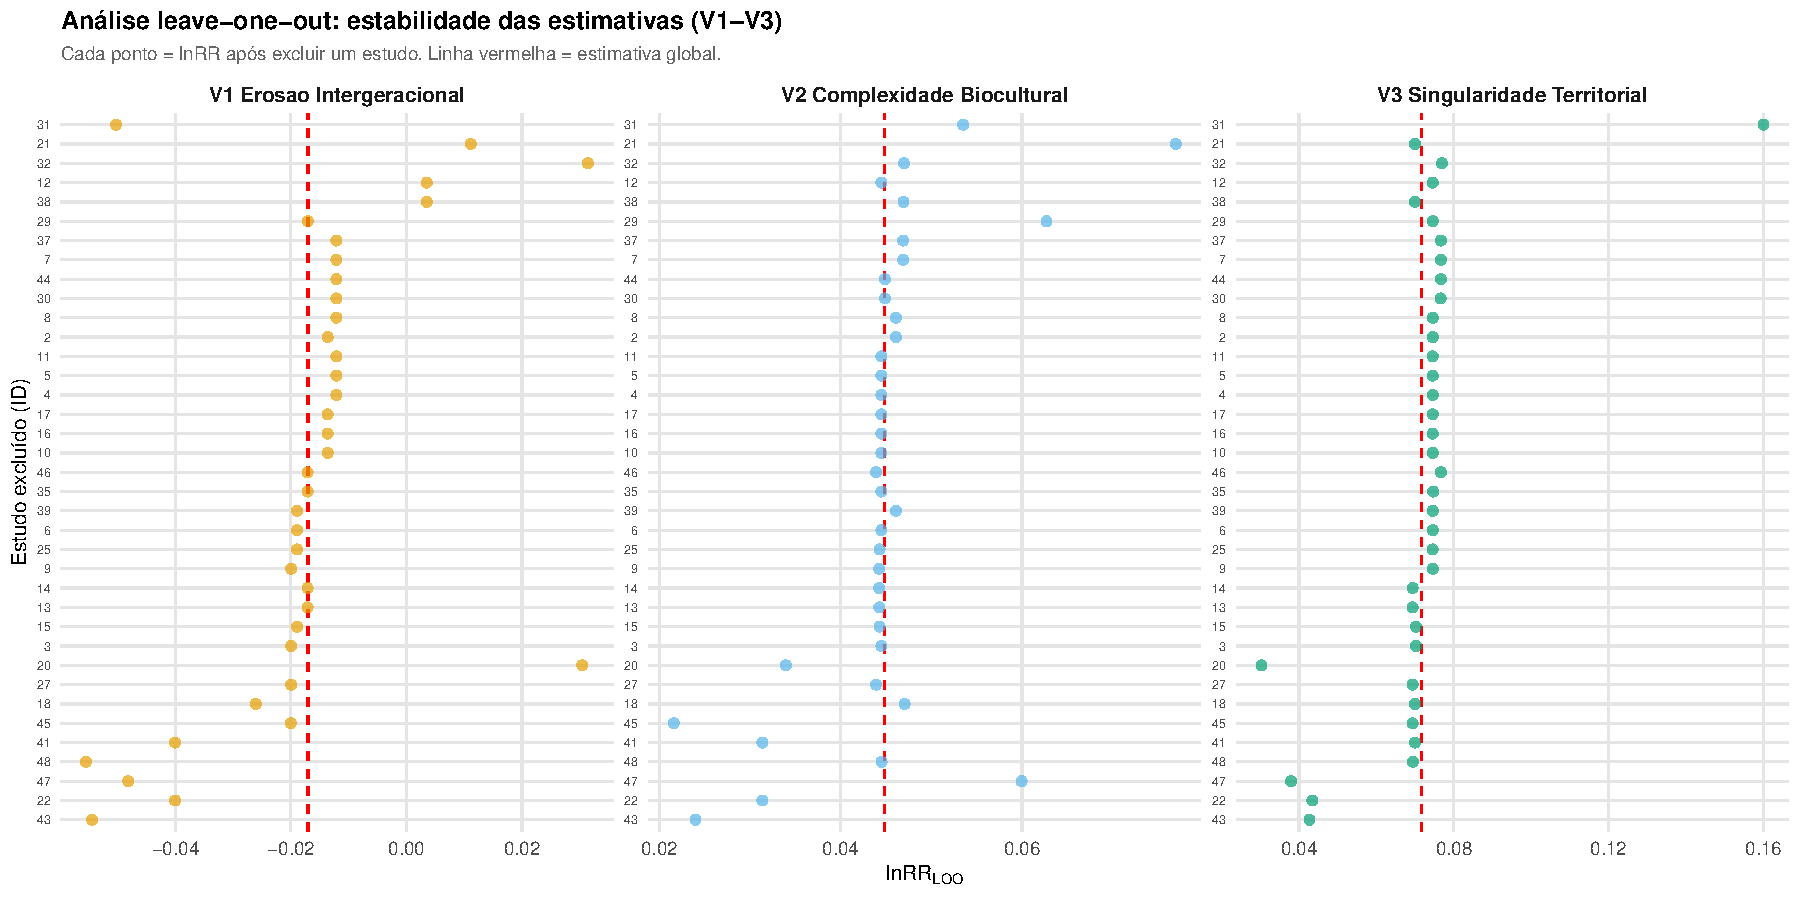
\includegraphics[width=\textwidth]{3-FIGURAS/leave_one_out_V1_V3.pdf}
  \caption{Dimensions $V_1$--$V_3$: intergenerational erosion, biocultural complexity, and documentation status}
  \label{fig:loo-a}
\end{subfigure}

\vspace{0.2cm}

\begin{subfigure}[b]{0.78\textwidth}
  \centering
  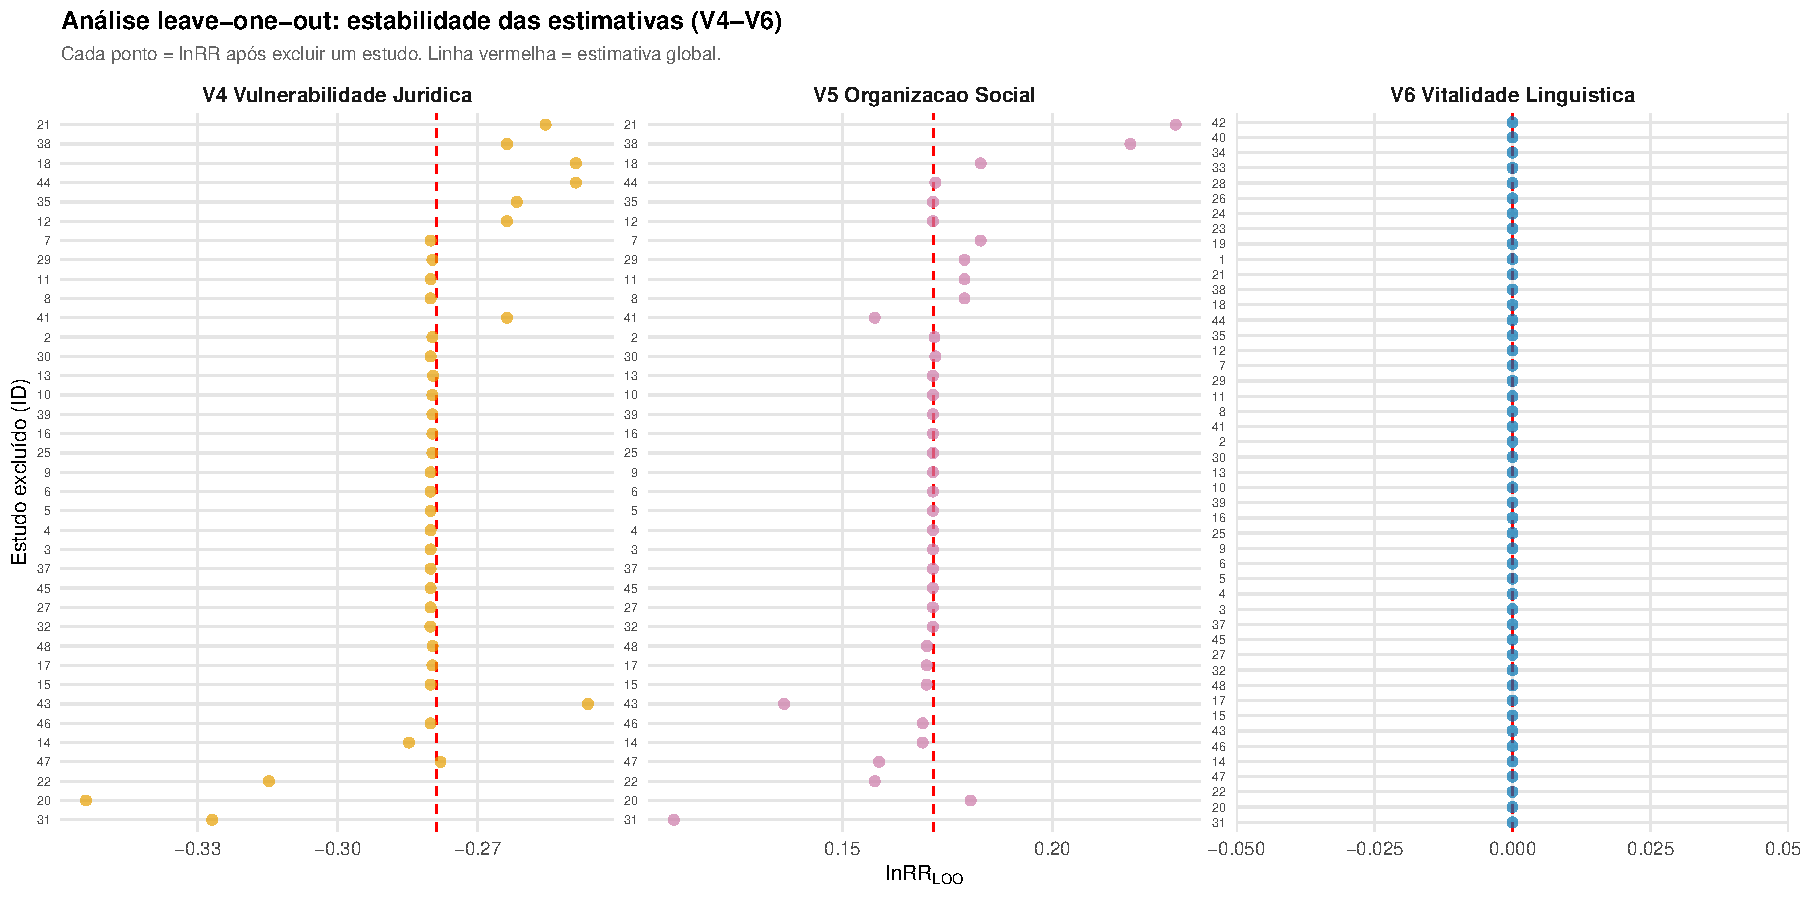
\includegraphics[width=\textwidth]{3-FIGURAS/leave_one_out_V4_V6.pdf}
  \caption{Dimensions $V_4$--$V_6$: legal vulnerability, social organization, and linguistic vitality}
  \label{fig:loo-b}
\end{subfigure}

\vspace{0.2cm}

\begin{subfigure}[b]{0.78\textwidth}
  \centering
  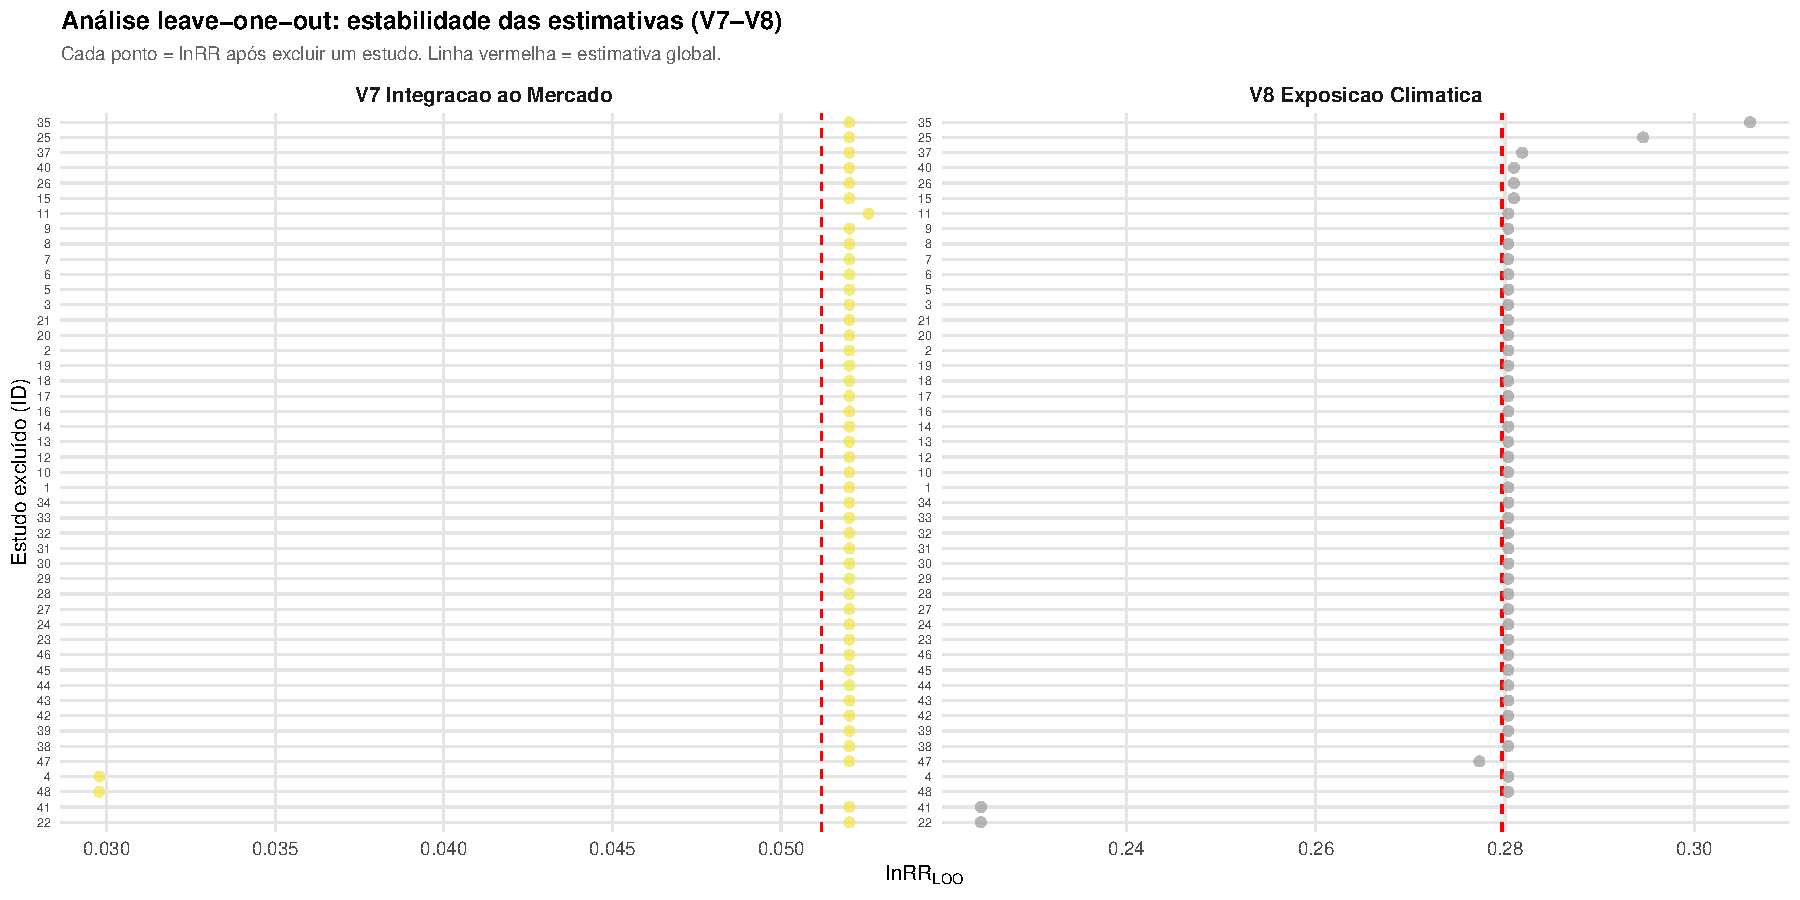
\includegraphics[width=\textwidth]{3-FIGURAS/leave_one_out_V7_V8.pdf}
  \caption{Dimensions $V_7$--$V_8$: market integration and climatic exposure}
  \label{fig:loo-c}
\end{subfigure}
\caption{Leave-one-out analysis: stability of \texorpdfstring{$\overline{lnRR}$}{lnRR} estimates after sequential exclusion of each study. (a) Dimensions $V_1$--$V_3$. (b) Dimensions $V_4$--$V_6$. (c) Dimensions $V_7$--$V_8$. The dashed red line indicates the overall estimate with all studies included}
\label{fig:loo}
\end{figure}

\subsection{The paradox of recognized but unmeasured vulnerability}
\label{sec:thematic-profile}

The corpus of 48 records is concentrated in \textit{traditional knowledge}, \textit{biocultural diversity}, \textit{agrobiodiversity}, and \textit{ethnobotany}, confirming the adequacy of the PICOS filtering to the intersection between local ecological knowledge and conservation. This thematic cohesion masks, however, an epistemological disjunction, as virtually all records acknowledge threats to traditional knowledge \citep{Mobarak2025,LaRosa2021,Suwardi2025,Essien2025}, yet only 7 of 48 (14.6\%) employ ``vulnerability'' as a research variable, and only \citet{Zeleke2025} operationalizes the concept with a framework of 15 indicators structured around exposure, sensitivity, and adaptive capacity.

The proportion of 31 qualitative to 17 quantitative studies (64.6\% vs.\ 35.4\%) confirms that biocultural vulnerability remains methodologically underoperationalized, a phenomenon attributable to ethnographic traditions that treat quantification with caution due to the risk of decontextualization \citep{Agrawal2002}. This gap is particularly relevant because the taxonomy of threats to traditional ecological knowledge proposed by \citet{TangGavin2016} identifies multiple and interactive pressure vectors whose operationalization requires composite indicators, while the scientific alert by \citet{FernandezLlamazares2021} documents the global convergence of threats on indigenous knowledge systems without offering standardized measurement metrics. The present meta-analysis seeks to fill this methodological gap between the descriptive corpus and the quantification necessary to inform safeguarding decisions.

\subsection{Intergenerational erosion as a nexus variable}
\label{sec:dimensional-coverage}

Among the eight proposed vulnerability dimensions ($V_1$--$V_8$), intergenerational erosion ($V_1$) is distinguished in the corpus reading not as a dimension equivalent to the others, but as the mechanism through which all others are reproduced or collapse. Twelve of the 48 studies explicitly document knowledge transfer processes, and the diversity of investigated contexts indicates that transmission is not a singular act but a system of distributed practices that assumes distinct forms depending on the ecosystem, gender, and community structure.

\citet{Cantor2025} demonstrates that the knowledge necessary for cooperative fishing with dolphins on the Brazilian coast is transmitted through situated learning, whose disruption implies not only loss of technical knowledge but dissolution of a coevolved interspecific relationship. \citet{Sibanda2025} shows that women's custodianship of landrace seeds in Zimbabwe simultaneously sustains household food sovereignty, cultural identity, and intergenerational knowledge transmission, such that seed vulnerability and epistemic vulnerability are, in this context, the same variable. \citet{Gerner2025} reveals that the preservation of medicinal plant knowledge in Europe depends on community social dynamics whose weakening through migration disrupts informal transfer mechanisms.

These studies, taken together, indicate that intergenerational transmission does not operate as a compartmentalized dimension but as a mediating variable whose failure may precipitate the decline of the remaining dimensions. This interpretation is consistent with longitudinal evidence of traditional knowledge loss in contemporary societies \citep{ReyesGarcia2013evidence}, with documented erosion in Maasai pastoral contexts \citep{HedgesKipila2020}, and among the Tsimane' \citep{Gruberg2022}, suggesting that the phenomenon transcends geographic and cultural boundaries. The co-occurrence of exogenous pressure vectors (migration, urbanization, market integration) and knowledge erosion supports this interpretation, insofar as \citet{Tran2025} documents how relocation policies in Vietnam disarticulate community networks of traditional water management, \citet{Moller2023} identifies emigration as the primary vector of ecological knowledge loss in South African rural communities, and \citet{Aniah2019} demonstrates that climatic variability in northern Ghana forces the adoption of alternative subsistence strategies that compete with the transmission of traditional agricultural practices.

This functional centrality of $V_1$ has direct implications for the interpretation of effect magnitude rankings and for the eventual construction of composite vulnerability assessment instruments. If intergenerational erosion operates as a causal nexus between exogenous pressures and the decay of all dimensions, treating it with symmetric weight to the others would underestimate its actual contribution to aggregate vulnerability, which should be considered in subsequent modeling studies. The near-zero effect observed for $V_1$ ($\overline{lnRR} = -0.017$) does not contradict this centrality, as it reflects the counterbalancing between communities where transmission is actively reinforced by safeguarding interventions and communities where collapse has already taken hold, canceling the aggregate effect.

The documentation status dimension ($V_3$) exhibited a near-zero effect ($\overline{lnRR} = +0.007$; $I^2 = 7.6\%$), yet meta-regression revealed individual coefficients that illuminate the internal dynamics of this dimension. Ecological knowledge indicators exhibited a positive trend ($\beta = +0.513$; $p < 0.001$), capturing formal registration processes where structured inventories and digitization protocols transform tacit knowledge into auditable documentation \citep{Zeleke2025,Suwardi2025}, while ethnobotanical assessments ($\beta = -0.405$; $p < 0.001$), agrobiodiversity assessments ($\beta = -0.405$; $p < 0.001$), and agroforestry assessments ($\beta = -1.078$; $p = 0.075$) suggested a protective effect, indicating that holistic documentation approaches better preserve the functional relationships between practices, territories, and transmission agents \citep{Maina2012,Poorna2014}. Digital preservation initiatives for indigenous knowledge systems \citep{Balogun2021} reinforce that effective documentation requires integration of audiovisual formats, contextual metadata, and community governance protocols.

The most evident gap in the corpus resides in the underoperationalization of legal vulnerability as a research variable. Although $V_4$ concentrates one of the two significant effects of the synthesis, none of the 48 primary studies employs ``legal vulnerability'' as an explicit variable, describing equivalent processes under fragmented terminologies such as ``erosion of biocultural diversity'' \citep{Mobarak2025}, ``loss of local and indigenous knowledge'' \citep{Suwardi2025}, and ``disappearance of oral history'' \citep{LaRosa2021}. This terminological dispersion suggests that an empirically relevant dimension remains conceptually diffuse, reinforcing the need for unified analytical frameworks such as the one proposed here. The scarcity of operationalization is noteworthy given that the existing literature on intellectual property \citep{Dutfield2004} and biocultural jurisprudence \citep{BavikatteRobinson2011,Nemoga2022} already offers theoretical and practical pathways for measuring legal vulnerability.

Climatic exposure ($V_8$), the second significant effect of the synthesis ($\overline{lnRR} = +0.280$; 95\% CI: $[0.03;\; 0.53]$), indicates that communities subjected to greater rainfall variability and frequency of extreme events tend to exhibit biocultural vulnerability indicators 32.3\% higher. The homogeneity of this estimate ($I^2 \approx 0$; 95\% PI: $[0.04;\; 0.52]$) suggests that the effect operates consistently across distinct geographic and cultural contexts, differing from the regionally heterogeneous pattern observed for $V_4$. This result is compatible with evidence that climatic perturbations force the substitution of traditional cropping calendars with alternative subsistence strategies that compete directly with the transmission of agricultural knowledge, promote the loss of local varieties adapted to historical rainfall regimes \citep{Savo2016}, and can disarticulate community water management networks whose functioning depends on contextual ecological knowledge. The interaction between climatic pressure and intergenerational discontinuity reinforces the interpretation of $V_1$ as a mediating variable, insofar as the perceived reduced practical relevance of traditional knowledge under altered climatic regimes may accelerate the abandonment of vertical transmission. Market integration ($V_7$, $\overline{lnRR} = +0.051$) exhibited a marginal trend of 5.3\%, compatible with the hypothesis that the progressive replacement of landrace varieties by commercial cultivars constitutes a vector of biocultural erosion whose magnitude, however, remains lower than that of climatic and institutional pressure in the analyzed corpus.

\subsection{Implications for vulnerability assessment and extraction targeting}
\label{sec:vulnerability-implications}

South American farming communities exhibited the greatest legal vulnerability ($\overline{lnRR} = -0.464$ for region, $-0.395$ for community type), suggesting that interventions to strengthen tenure regimes and formal heritage registration may be prioritized in these contexts. Strategies anchored in symbolic territories (sacred groves, ceremonial areas) exhibited the highest protective coefficients ($\beta_{V5} = +1.496$; $\beta_{V6} = +1.407$), suggesting that the integration of ritual practices and institutional visibility may produce simultaneous effects on social cohesion and cultural vitality, a result compatible with the reconceptualization of community conservation proposed by \citet{Berkes2004} and with adaptive co-management as a resilience-building mechanism \citep{OlssonFolkeBerkes2004}. Mitigation of climatic exposure ($V_8$) constitutes the fourth axis, given that the consistency of the effect across contexts ($I^2 \approx 0$) suggests that the vulnerability associated with extreme events operates as a cross-cutting pressure whose response may require the integration of climate adaptation and traditional knowledge safeguarding. Approaches centered exclusively on isolated ecological indicators ($\beta_{V5} = -0.919$) not only were not associated with protective effects but may have captured erosive processes already underway.

The methodological composition of the corpus (64.6\% qualitative studies) reflects an epistemological tension inherent to the field, in which the quantification of tacit and relational knowledge faces legitimate objections regarding reification \citep{Agrawal2002,GomezBaggethun2013}. The strategy adopted in this meta-analysis partially addresses this tension by anchoring estimates in response ratios with explicit uncertainty propagation and by maintaining $I^2$ as an interpretive caution parameter.

The identification of gender as a cross-cutting theme in eight studies (16.7\%) suggests that this moderator may be relevant for understanding biocultural vulnerability and merits investigation in future meta-regressions. \citet{RomeroSilva2026} documents the role of women in agrobiodiversity conservation in Mesoamerican homegardens, and \citet{MugiNgenga2016} identifies gender asymmetries in agricultural intensification, signaling that communities with greater female participation in knowledge governance may exhibit distinct effect magnitudes for $V_1$ (intergenerational erosion) and $V_3$ (documentation status).


\subsection{Moderators and estimate stability}
\label{sec:moderadores-discussao}

South America and Asia concentrate the significant negative effects for $V_4$ (Fig.~\ref{fig:meta-reg-regiao}), revealing a continental gradient of legal vulnerability consistent with contexts where land tenure pressure on traditional territories converges with institutional fragility, accelerating the erosion of legal protection frameworks. In the African and European regions, however, confidence intervals remain compatible with neutrality, suggesting that regional protective factors operate as buffers against documentation erosion. In Zimbabwe, the community seed custodianship documented by \citet{Sibanda2025} exemplifies this compensatory mechanism, while the European ethnobotanical networks described by \citet{Gerner2025} represent functionally analogous safeguarding structures. The resilience of agricultural knowledge systems in Iberian homegardens \citep{ReyesGarcia2014} and the integration of context-specific knowledge in the recovery of culturally significant species \citep{Rayne2022} illustrate how biocultural complexity ($V_2$) can operate as a protective factor when preserved. This geographic asymmetry suggests that protection policies may benefit from regional calibration, prioritizing Latin America and Southeast Asia.

Traditional farming communities exhibit the greatest legal fragility ($\overline{lnRR} = -0.395$, Fig.~\ref{fig:meta-reg-comunidade}), surpassing both indigenous ($\overline{lnRR} = -0.241$) and rural communities ($\overline{lnRR} = -0.156$). This difference suggests that the legal protection mechanisms available to indigenous peoples, including intellectual property regulatory frameworks and Nagoya protocols \citep{BavikatteRobinson2011,Robinson2014}, provide partial protection that does not extend to traditional farming communities lacking formal ethno-territorial recognition. In contrast, the positive trend for $V_5$ in rural communities ($\overline{lnRR} = +0.688$), although without statistical significance, points to collective organization as a possible compensatory mechanism in the face of vulnerability in other dimensions, a result compatible with the hypothesis that social learning and the evolution of conservation practices depend on adaptive governance networks \citep{BerkesTurner2006,Folke2004}.

Interventions anchored in symbolic territories, such as sacred grove conservation (Fig.~\ref{fig:meta-reg-intervencao}), emerged as the moderator with the greatest simultaneous protective effect on $V_5$ ($\beta = +1.496$; $p = 0.014$) and $V_6$ ($\beta = +1.407$; $p = 0.001$), indicating that territorially rooted practices can produce synergistic effects on social cohesion and cultural vitality. Ecological knowledge indicators, in contrast, exhibited a negative effect on $V_5$ ($\beta = -0.919$; $p < 0.001$), suggesting that this type of measurement may capture erosive processes already underway. These contrasts reinforce the need to distinguish between ex situ interventions focused on monitoring and cataloging, and in situ interventions aimed at strengthening territorial practices \citep{Zimmerer2018}, in the formulation of safeguarding strategies. The interdependence between linguistic extinction and loss of unique medicinal knowledge \citep{CamaraLeret2021} reinforces that biocultural complexity ($V_2$) cannot be assessed in isolation from the dimensions of social organization and linguistic vitality.

No individual exclusion reversed the direction or significance of effects across the eight dimensions (Fig.~\ref{fig:loo}). For $V_4$ (legal vulnerability), no individual exclusion reversed the direction of the negative effect ($\Delta_{\max} = 0.075$), and the removal of \citet{Sibanda2025}, the study with the largest sample weight, deepened the estimate from $-0.279$ to $-0.354$, indicating that the result does not depend on a single influential study. For $V_3$ (documentation status), the greatest observed sensitivity ($\Delta_{\max} = 0.077$) remained modest relative to the near-zero effect, without altering the direction of the estimate. For $V_2$ (biocultural complexity), the low sensitivity to exclusion ($\Delta_{\max} = 0.028$) aligns with the low heterogeneity ($I^2 = 3.6\%$), indicating the dimension with the most homogeneously distributed effect across studies.

\subsection{Limitations}
\label{sec:limitations}

Given the meta-analytic nature of this research, it is pertinent to acknowledge certain limitations. One pertains to the predominance of qualitative evidence in the corpus (74.5\% of records classified as Tier~3 or Tier~4), meaning that most effect sizes derive from ordinal conversions; however, the tier-specific variance inflation was designed to accommodate this uncertainty, and results remained stable in sensitivity analysis. Another potential limitation concerns the reduced sample sizes in some stratifications by region and community type ($k = 1$--$12$), which may restrict the transferability of findings to unrepresented contexts. Nevertheless, the observed patterns are consistent with the literature and provide a basis for hypothesis formulation in future investigations.


%% ============================================================
%% 5. CONCLUSION
%% ============================================================
\section{Conclusion}
\label{sec:conclusions}

The results indicate that institutional fragility, operationalized through legal and land tenure vulnerability ($V_4$), and climatic exposure ($V_8$) constitute the two significant vectors of biocultural degradation in traditional agricultural knowledge and systems, whereas ecological, documentation, and biocultural complexity indicators exhibited near-zero effects. Legal vulnerability was concentrated in South American traditional farming communities, where the disconnect between customary tenure regimes and national regulatory frameworks accentuates the erosion of protection mechanisms, while climatic exposure operated homogeneously across geographic and cultural contexts, suggesting that extreme event pressure constitutes a cross-cutting degradation vector. Intergenerational transmission ($V_1$) operates as a mediating variable whose failure may precipitate the simultaneous decline of the remaining dimensions, signaling that the continuity of these systems depends more on the maintenance of legal, territorial, and social conditions than on the volume of documented knowledge. Interventions anchored in symbolic territories exhibited the highest simultaneous protective coefficients for social organization ($V_5$) and linguistic vitality ($V_6$), indicating that safeguarding policies may benefit from the integration of legal-land tenure reinforcement, strengthening of community organization, and climate adaptation.

%% ============================================================
%% Acknowledgments
%% ============================================================
\section*{Acknowledgments}

The authors thank the Graduate Program in Intellectual Property Sciences (PPGPI/UFS) for institutional support. This study was supported by the Conselho Nacional de Desenvolvimento Cient\'{i}fico e Tecnol\'{o}gico (CNPq) and the Funda\c{c}\~{a}o de Amparo \`{a} Pesquisa do Estado da Bahia (FAPESB).


%% ============================================================
%% SUPPLEMENTARY MATERIAL
%% ============================================================
\section*{Supplementary Material}

The Supplementary Material associated with this article can be found in the online version at [DOI to be inserted]. The document contains: Online Resource~1 -- PRISMA flow diagram detailing the study selection process; Online Resource~2 -- Table of meta-analysis results by biocultural vulnerability dimension ($k = 37$--$47$ studies, \texttt{rma.mv} model with REML and RVE-CR2, $\rho = 0.8$), including prediction intervals; Online Resource~3 -- Mapping table between meta-analytic indicators and functional dimensions; Online Resource~4 -- Feasibility diagnosis table by dimension.

%% ============================================================
%% REFERENCES
%% ============================================================
\bibliographystyle{plainnat}    %% natbib author-year (Springer compatible)
\bibliography{references}


%% ============================================================
%% STATEMENTS AND DECLARATIONS (after References per B&C guidelines)
%% ============================================================
\section*{Statements and Declarations}

\subsection*{Funding}

This study was financed in part by the Coordena\c{c}\~ao de Aperfei\c{c}oamento de Pessoal de N\'ivel Superior -- Brazil (CAPES).

\subsection*{Competing Interests}

The authors declare that they have no known competing financial interests or personal relationships that could have appeared to influence the work reported in this article.

\subsection*{Author Contributions}

\textbf{Catuxe Varj\~ao de Santana Oliveira:} Conceptualization, Methodology, Investigation, Formal analysis, Data curation, Writing -- original draft.
\textbf{Luiz Diego Vidal Santos:} Methodology, Formal analysis, Validation, Writing -- review \& editing.
\textbf{Paulo Roberto Gagliardi:} Writing -- review \& editing, Supervision.
\textbf{T\^ania Cristina Azevedo:} Writing -- review \& editing.
\textbf{Renisson Neponuceno de Ara\'ujo Filho:} Writing -- review \& editing.
\textbf{Francisco Sandro Rodrigues Holanda:} Writing -- review \& editing.

\subsection*{Data Availability}

The extraction dataset, analysis scripts, and meta-analytic outputs are available on Mendeley Data (\url{https://doi.org/10.17632/mh5sbx7ky7.1}).

\end{document}
